% Document class, language and encoding setup
\documentclass[a4paper,12pt,english]{report}

\usepackage[english]{babel}
\usepackage[utf8]{inputenc}
\usepackage[T1]{fontenc}
% Fixing the font issue
\usepackage{ae,aecompl}

% Color package
\PassOptionsToPackage{dvipsnames}{xcolor}
	\RequirePackage{xcolor} % [dvipsnames] 
	
% Allows page-links in pdf file
\usepackage{hyperref}
\hypersetup{
% Uncomment the line below to remove all links (to references, figures, tables, etc)
%draft, 
%colorlinks=true, linktocpage=true, pdfstartpage=3, pdfstartview=FitV,
% Uncomment the line below if you want to have black links (e.g. for printing black and white)
colorlinks=true, linktocpage=true, pdfborder={0 0 0}, 
pdfstartpage=3, pdfstartview=FitV, hypertexnames=true, pdfhighlight=/O, 
breaklinks=true, pdfpagemode=UseNone, pageanchor=true, pdfpagemode=UseOutlines, plainpages=false,
bookmarksnumbered, bookmarksopen=true, bookmarksopenlevel=1,
urlcolor=Black, linkcolor=Black, citecolor=Black,
%------------------------------------------------
% PDF file meta-information
%pdftitle={\myTitle},
%pdfauthor={\textcopyright\ \myName, \myUni, \myFaculty},
%pdfsubject={},
%pdfkeywords={},
%pdfcreator={pdfLaTeX},
%pdfproducer={LaTeX with hyperref and classicthesis}
%------------------------------------------------
} 

\usepackage{pdfpages}
% Todo notes package and commands
\usepackage{todonotes}
% Allows commands to emit a space "at the end"
\usepackage{xspace}
%tabularextension
\usepackage{longtable}
% Listings setup
\usepackage{listings}

% Graphics setup
\usepackage{graphicx}
\graphicspath{{./graphics/} {./graphics/sprint1/}}

\usepackage{tikz}
\usetikzlibrary{calc}
\usetikzlibrary{arrows,backgrounds,snakes}

\usepackage{tikz-uml}

\usepackage{amsmath}
\usepackage{amssymb}

% Advanced tables
\usepackage{tabularx}
\usepackage{multirow}

% Clever references
\usepackage{cleveref}

% Named references
\usepackage{nameref}

% Bibliography
\usepackage[square,numbers]{natbib}
\bibliographystyle{unsrt}

% Force position [H]
\usepackage{float}

% For figures with sub-figures
\usepackage{subcaption}

% Caption package. Makes label of caption bold.
\usepackage[labelfont=bf]{caption}

% Additional commands
\newcommand{\namedtodo}[5]
{
  \ifthenelse{\equal{#1}{}}
  {
    \todo[backgroundcolor=#4,caption=
    {\textbf{#3: } #2}
    ,inline]
    {\color{#5}\textbf{#3: }#2}
  }
  {
    \todo[backgroundcolor=#4,caption=
    {\textbf{#3: } #1}
    ,inline]
    {\color{#5}\textbf{#3: }#2}
  }
}
\newcommand{\mikkel}[2][]{\namedtodo{#1}{#2}{Mikkel}{blue!80}{white}}
\newcommand{\stefan}[2][]{\namedtodo{#1}{#2}{Stefan M}{orange}{black}}
\newcommand{\anders}[2][]{\namedtodo{#1}{#2}{Anders}{orange}{black}}
\newcommand{\thilemann}[2][]{\namedtodo{#1}{#2}{Stefan T}{NavyBlue!35}{NavyBlue}}
\newcommand{\mikael}[2][]{\namedtodo{#1}{#2}{Mikael}{green}{black}}
\newcommand{\bruno}[2][]{\namedtodo{#1}{#2}{Bruno}{black!10!red!90}{white}}
% Her er en liste over navnene på de forskellige styles
% C#: csharp
% F#: fsharp

% 
% Listings kan refereres vha. \cref{}
\crefname{listing}{code example}{code example}
\Crefname{listing}{Code example}{code examples}
% 

%Algoritmer i cref
\crefname{algocf}{algorithm}{algorithm}
\Crefname{algocf}{Algorithm}{Algorithms}
%

% Angivelse af navn på listings
\renewcommand\lstlistingname{Code example}
\renewcommand\lstlistlistingname{Code example}

\lstdefinestyle{standard}
{
	frame=shadowbox,
	framesep=5pt,
	rulecolor=\color{blue!40!black},
	rulesepcolor=\color{white!93!black},
	numbers=left,
	basicstyle=\ttfamily,
	numberstyle=\tiny,
	numberfirstline=true,
	%numberblanklines=false,
	stepnumber=1,
	numbersep=9pt,	
	captionpos=b,
	escapeinside={(*}{*)},
	breaklines=true,
	tabsize=4,
	language=c
}

\lstset{style=standard}

\lstdefinestyle{c}
{
	style=standard
}

\lstdefinestyle{csmall}
{
	style=c
}

\lstdefinestyle{csharp}
{
	style=standard,
	language=[Sharp]C
}
\lstdefinestyle{csharpsmall}
{
	style=csharp
}
\lstdefinestyle{fsharp}
{
	language=[Sharp]F,
	frame=lr,
	rulecolor=\color{blue!80!black}
}
\lstdefinestyle{fsharpsmall}
{
	style=fsharp,
	basicstyle=\ttfamily\footnotesize
}


%Definitions
\newcommand{\mindsqualls}{MindSqualls\xspace}
\newcommand{\csharp}{\textsc{C\#}\xspace}
\newcommand{\fsharp}{\textsc{F\#}\xspace}
\newcommand{\legoms}{Lego Mindstorms\xspace}
%\newcommand{\lego}{\textsc{LEGO$^{\textrm{\scriptsize\textregistered}}$}\xspace}
\newcommand{\lego}{Lego\xspace}
\newcommand{\legos}{Legos\xspace}
\newcommand{\kinect}{Kinect\xspace}

%Superscript and subscript
\newcommand{\superscript}[1]{\ensuremath{^{\textrm{#1}}}}
\newcommand{\subscript}[1]{\ensuremath{_{\textrm{#1}}}}

% Degrees
\newcommand{\degree}{\ensuremath{^\circ}}
\newcommand{\dg}{\degree}

\newcommand{\quoter}[1]%
{
  \par
  \vspace{1.5em}
  \addtolength{\leftskip}{1.5cm}
  \addtolength{\rightskip}{1.5cm}
  \textit{#1}
  \addtolength{\leftskip}{-1.5cm}
  \addtolength{\rightskip}{-1.5cm}
  \vspace{1.5em}
  \par
}

% For fancy pseudocode algoritms
\usepackage[algochapter,lined,boxed,noend]{algorithm2e}
\renewcommand{\listalgorithmcfname}{Liste over Algoritmer}
\renewcommand{\algorithmcfname}{Algoritme}
\renewcommand{\algorithmautorefname}{algoritme}
\renewcommand{\algorithmcflinename}{linje}

% Math proofs and stuff.
\usepackage{amsthm}
\usepackage{bigints}

\newcommand{\HRule}{\rule{\linewidth}{0.5mm}}
\begin{document}
%Front page
\begin{titlepage}

\begin{center}

\HRule \\[0.4cm]
\textsc{ \Huge GIRAF \\[0.3cm]
	\Large Cars Voice Game }\\[0.4cm]

\HRule \\[1cm]

\textsc{\Large SW613F14} \\[2cm]


\includegraphics[width = \textwidth/2]{ic_launcher}

\vfill
{\Large Developing Complex Software Systems}
\\ ~\\
{\large Spring Semester 2014}

\end{center}
\end{titlepage}

\pagenumbering{Roman}
\setcounter{page}{1}
\setcounter{secnumdepth}{3}

\thispagestyle{empty}
\phantom{p. 1}
\clearpage

\thispagestyle{empty}
\begin{titlepage}
\begin{nopagebreak}
{\samepage 
\begin{tabular}{r}
	\parbox{16cm}{\raisebox{11mm}{
\includegraphics[height=1.2cm]{aauLogoEn.jpg}}
	\hfill \parbox{7cm}{\begin{tabular}{l}
		{\small \textbf{Department of Computer Science}}\\
		{\small Selma Lagerløfs Vej 300} \\
		{\small 9220 Aalborg Ø} \\
		{\small Phone (+45) 9940 9940} \\
		{\small Fax (+45) 9940 9798} \\
		{\small http://cs.aau.dk}
	\end{tabular}}
	}
\end{tabular}

\begin{tabular}{cc}
	\parbox{8cm}{
	\begin{description}
		\item { \textbf{Title:}}\\ 
			Cars Audio Game
    		\item { \textbf{Subject:}}\\ 
			\raggedright Developing Complex Software Systems
	\end{description}
	
	\parbox{8cm}{
	\begin{description}
		\item { \textbf{Project period:}}\\
			03-02-2014 -\\
			28-05-2014
 		\hspace{4cm}
		\item { \textbf{Project group:}}\\
  			sw613f1f
 		\hspace{4cm}
		\item {\textbf{Participants:}}\\
			Bruno Thalmann\\
			Mikael E. Christensen\\
			Mikkel S. Larsen\\
			Stefan M. G. Micheelsen\\
		\hspace{2cm}
		\item { \textbf{Supervisor:}}\\
 			Thomas Pedersen\\
  	\end{description}
	}
	\begin{description}
		\item { \textbf{Printings:} X}
		\item { \textbf{Pages:} X } 
		\item { \textbf{Appendices:} X}
		\item { \textbf{Total pages:} X }
		\item { \textbf{Source code:} X}
	\end{description}
	\vfill } &
	\parbox{6.5cm}{
 	 \vspace{.15cm}
  	\hfill 
  	\begin{tabular}{l}
  		{ Abstract:}\bigskip \\
  		\fbox{
  		\parbox{6cm}{\bigskip
     		{\vfill{\small This project is a part of a multi-project, consisting of 16 groups, from Software-Engineering 6th semester at Aalborg University.
The purpose of the multi-project is to develop a series of applications for autistic people.

The focus of the project-group is a game that should help in improving the auditory sense.
In the game you must control a car, moving from the left to the right, while avoiding or collecting objects.
The car is manoeuvred up and down by the volume of the speech produced by the player.

A speech therapist and two pedagogues from Aalborg Kommune are the main stakeholders of this product.
Throughout the project there has been meeting with the customers to match expectations and manufacture requirements.

To contribute to the multi-project process, the report also contains two chapters to be used by future multi-projects. The first chapter contains a description of the generic framework used to develop the game.
The second chapter is about the git usage in the multi-project, with a detailed explanation of the usage and common mistakes.
     		\bigskip}}
     	}}
   	\end{tabular}}
\end{tabular}
}%samepage end
\\
\vfill
\noindent{\footnotesize{\textit{The content of this report is freely available, but if published it has to be acknowledged by
the authors.}}}
\end{nopagebreak}
\end{titlepage}
\clearpage

\newcommand{\prefaceHeaderName}{Preface}
\section*{\prefaceHeaderName}
This report has been made by 6th semester Software-Engineering students at Aalborg University, during the spring-semester of 2014.
It is expected of the reader to have a background in IT/software, due to the technical content.

References and citations are done by the use of numeric notation, e.g. \cite{music-and-computers}, which refers to the first item in the bibliography.
Whenever the report refers to 'we', it is to be understood as the members of the project-group.

On the following page, a glossary can be found, containing words and terms that might not be apparent from their context when used in the report.

We would like to thank our lecturers, as well as our supervisor Thomas Pedersen, for his guidance throughout the semester.
\newpage

\newcommand{\glossaryHeaderName}{Glossary}
\section*{\glossaryHeaderName}
\begin{description}
\item[Citizen] A person with autism.
\item[Legal Guardian] The legal guardian of a citizen.
\item[Institutional Guardian] An employee from an institution responsible for citizens.
\item[Pictogram] Is a symbol in the form of a simplified drawing, that is used to inform, instruct or caution.
\end{description}

\clearpage

%Table of content
\pdfbookmark{\contentsname}{toc}
\setcounter{tocdepth}{1}
\tableofcontents

\clearpage

\pagenumbering{arabic}

\newcommand{\introductionHeaderName}{Introduction}
\chapter*{\introductionHeaderName}
\addcontentsline{toc}{chapter}{\introductionHeaderName}
Throughout the entire course of this multi-project, the project-group worked on a project called Stemmespillet (formerly Cars).

The overall structure and purpose of the project is explained in \cref{multiproject}, along with the project's place in multi-project.

The multi-project was divided into 4 sprints, each with its own process and result.
The result of each sprint is documented by a chapter (see chapters \ref{sprint1}-\ref{sprint4}).

As another result of the project, two chapters were formed, to be used by next year's multi-project semester.
The first chapter contains a description of a generic Android Game Framework, which could be the foundation for new games.
The second chapter contains a guide to the way version control, by the use of Git, was handled during the semester.

As a conclusion of the report, some general advice will be given, to be used by next year's multi-project.

\chapter{Multi-project}\label{multiproject}

\section{GIRAF}

\textit{Graphical Interface Resources for Autistic Folk} (GIRAF) is a semester-wide multi-project collaboration between all Software 6th semester (SW6) groups at Aalborg University.
The project started with the SW6 students of 2011 and has run every year since then (this being the 4th year).

The overall idea of the project is to create a multi-purpose Android application, which can be used to ease the lives of citizens and their institutional guardians.
The main goal is to recreate already existing physical tools/methods in digitalized versions.
Additionally, in order to make it an all-use-and-purposes application, it will also serve as an administration tool for each individual institution that will put it to use.

GIRAF is run in collaboration with Aalborg Municipality.
This year there is a total of 6 stakeholders (all institutional guardians or otherwise linked to institutions) who will be available during the course of the project.

\subsection{Applications}
The applications developed by GIRAF are assembled in the Launcher application.
The Launcher uses a QR-code as log in method.
It can also be used as a home-screen.
It is possible to log in as guardian.
When logged in it is possible to switch between two modes, guardian and citizen.
But it is only possible to switch to the citizens associated to the guardian logged in.
The Launcher contains all applications developed by GIRAF, which makes it possible to have as the only home-screen.
The Launcher for instance has an application to make pictograms, where it is possible to draw or take a picture and record a sound to make a pictogram.
Another application is an administration tool for handling adding and removing citizens and guardians.
There is also an application for week-planning which uses series of pictograms so show the citizen what to do.

\section{Organization}
The multi-project consists of 60 people split into 16 project-groups, each group consisting of 4 people (except for two groups, that was the split of a former 4-man group).

\subsection{Method}
Due to the high level of collaboration and the focus on getting out a usable and working product, an agile methodology was in mind when planning the process.
The method chosen was Scrum of Scrums.
Each project-group would work as a team, with their own day-to-day activities, focusing on their current project during the sprint.
Then there would be common weekly status meetings during the sprints, each sprint concluded with sprint-review and sprint-planning meetings.

\subsubsection{Sprints}
The semester was split into 4 sprints, with the last three sprints being of same length (The first was a bit shorter, as this was meant as a sprint solely for getting to know the former projects).
In order to take into consideration the courses that were running simultaneously with the multi-project, sprint lengths were based on available hours (with the subtraction of course hours).

At the end of each sprint, a sprint review meeting would be held, where all stakeholders were invited.
Here the current products (if possible) would be presented by each group and critiqued by stakeholders and the other groups.
Also, the product backlog would be presented for the stakeholders, in order to get some input on what to focus on in the following sprint.

Following the sprint review, and without the stakeholders, the next sprint would be planned.
Here groups had a chance to switch focus, if their current project was finished, or if something more important had presented itself as a result of the sprint review.

\subsubsection{Meetings}
In order to stay on top of potential problems, a status meeting was held every week (with exception of sprint-end weeks).
The meetings started out with a status report, where a representative from each group presented what they were currently working with, along with any potential problems that needed attention.

If there were problems, these were noted and the proper people informed, so that they could discuss these, without everyone needing to be part of the discussion.
This saved a lot of time, as opposed to having everyone discussing every problem.

However, subjects that did need to be discussed with all groups present would be added to the meeting agenda and then discussed at the meeting.

\subsubsection{Specialists}
In order for people to concentrate on their respective projects, a few people were named specialists in different areas (such as server, contact with stakeholders, and version control).
Each person were responsible for their area; that it was working as it should, as well as helping people with possible problems.

\subsection{Stakeholders}
Day-to-day contact with stakeholders went through a specialist (contact person).
As mentioned, all stakeholders were invited to each sprint review, where they would give feedback to the presented work as well as available for questions.
If any more contact was needed, such as arranging a meeting, this was conveyed by the contact person.

\subsection{Shared Components}\label{multiproject:sharedcomponents}
There were two main shared components; database and GUI components.

The database consisted of the storage of shared data, as well as providing an interface for accessing this data.

The GUI components consisted of shared graphical components, such as backgrounds, buttons and other things that were commonly used and needed to look the same across applications.

As an addition to the shared components, whenever needed, groups would collaborate on minor shared components that could be used across applications.

\subsection{Tools}
In the beginning of the project two representatives from the previous semester told about the tools they used on their semester and their experience with them.
Based on these experiences a couple of tools were chosen to aid the project.
These tools will be described in the following sections.

\subsubsection{Redmine}
Redmine was used as a center of information, consisting of three main uses; forums, wiki-pages, and issue-trackers.

The forums were used for non-pressing matters.
Here, updates to shared components were posted, along with possible instructions if changes needed to be applied to concerned projects.

Wiki-pages were used for static information.
There was a main wiki-page, containing group contact informations, general guides, and meeting summaries.
Additionally, each sub-project had the possibility for its own wiki-page, to contain whatever information about their project that needed to be shared with others.

Issue-tracking was a tool for tracking progress of a project, as well as the possibility to state issues for other projects that ones own project needed done.
Issue-tracking also made it easier for a group to take over the projects if they changed focus after a sprint.

\subsubsection{Git}
Git was used as version control.
Since one of the group members was the Git-specialist, this is the focus of one of the collaboration chapters (see \ref{collaboration:git}).
\bruno{Thomas: Man kunne evt. svare på følgende spørgsmål: - Hvad er fordelene med version kontrol?
- Er der nogle specielle grunde til at git blev foretrukket over andre muligheder?}
\mikael{Don't know what more to write here if anything.}

\subsubsection{Jenkins}
\mikael{Don't know what to exactly write here}.

\section{Cars}
Throughout the entire course of this project, the project-group has worked with an application called Stemmespillet (Translates to 'The Voice Game').
It was originally named 'Cars', but was changed to Stemmespillet midway through the multi-project.
However, Cars was kept as a working title, and the project will be mentioned as Cars throughout the report.
Cars is a sub-application of the GIRAF-application, with its own purpose; that of assisting citizens in learning to control their pitch of speech (This is explained in \cref{sprint1}).

\subsection{Collaboration with stakeholders}
In order to establish its overall purpose and to make it as useful as possible, there were three main stakeholders that were cooperated with during the project.
Two are institutional guardians at 'Birken', a home for psychologically disabled children, and the third is a speech therapist, associated with Aalborg Municipality.
These stakeholders were the most relevant for this sub-application, based on the citizens they worked with on a daily basis.
These were also the stakeholders with the most relevant input, both during interviews and sprint reviews.

\subsection{Collaboration with multi-project}
Cars is a sub-application of the GIRAF-application which needs to follow certain project-standards.
For Cars there were one overall standard; one for GUI.

Following GUI standards is necessary to give all the applications the same look and feel.
Cars will be updated to fulfil these standards in \cref{sprint3:gui}.

GIRAF also uses a common database to share data.
Data is shared for two purposes; re-acquiring saved data in case of replacement of the tablet, and for multi-user tablets.

The project group also had two responsibilities; Git and Redmine Wiki.
Each were assigned to one of the group members.
The first one took up a lot of time for the concerned person, which also led to the collaboration chapter on the subject of Git.
The latter did not take up a lot of time.

\mikael{Der skal skrives et underafsnit om vores metode i gruppen, SCRUM skal nævnes}

\chapter{Sprint 1}\label{sprint1}
In this sprint we focused on the 'Cars' project from last year's multi-project.
The main purpose of the sprint was to get an understanding of the project, while making it usable by eliminating bugs and implementing missing features.

Cars is a small game, in which the user controls a car, automatically moving from left to right on a three-lane road.
The user must use voice input, based on pitch, to move the car up and down in order to dodge obstacles on the road and in the end manoeuvre the car into a garage.
A screenshot from the Cars app can be seen in \cref{fig:cars_screenshot}.

\begin{figure}[h]
\centering
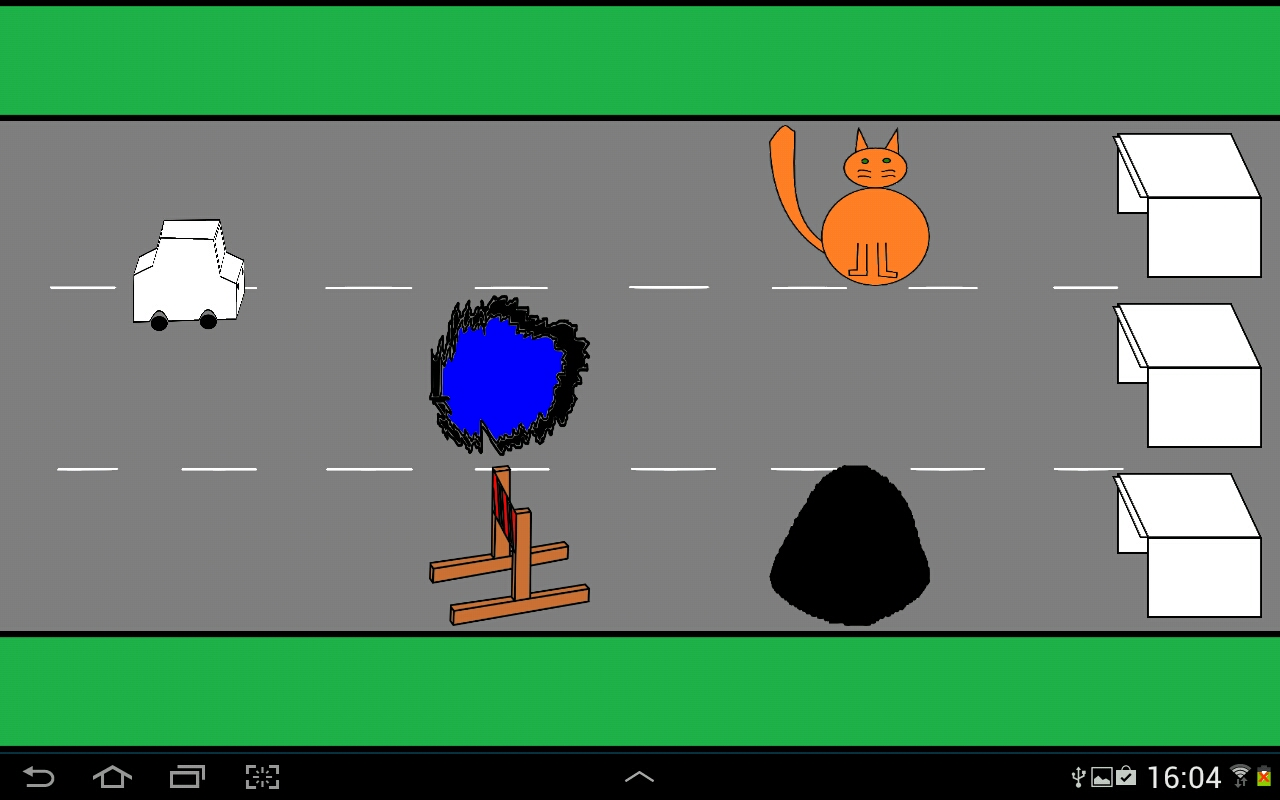
\includegraphics[width=.5\textwidth]{sprint1/cars_screenshot}
\caption{Screenshot from the 'Cars' app.}
\label{fig:cars_screenshot}
\end{figure}

Sound input is an important element of Cars, as it is used to control the car.
It was also a part of the game which did not work properly.
The car's movements did not correctly correspond to the voice input, seemingly causing the car to move at random, no matter what kind of pitch was used.

Using voice input based on pitch was an original requirement of the Cars project, worked out between the Cars group and the stakeholders.
Its intention was to solve a particular problem concerning some autists, not being able to control their pitch during speech.
Based on its importance and that it does not work, this would be a natural major focus point during the first sprint.

However, in the following two sections of this chapter, we will argue that there are two overall problems with trying to improve the already existing Cars project.
Firstly we will argue that it is very difficult to obtain frequency from sound input.
Secondly we will argue that it would be easier to completely reboot the Cars project, with new framework and structure, rather than continuing on the existing code and structure.

We will instead argue for using volume instead of pitch, after confirming its validity with the stakeholders.
Additionally we will propose a structure, based on the KiloBolt framework.
\newpage

\section{Product requirements}
\label{sprint1:requirements}

The first step in continuing on the project from last year was to collect the requirements that the old project group had used.
The following requirements are extracted from the report written by the old project group \citet*{oldcars}:

\begin{enumerate}
\item The game must not be a sidescrolling game, because the citizen must be able to see the goal
\item The game must make it possible for the citizen to control a car
\item The game should contain stars as points
\label{sprint1:requirements:points}
\item The goal of the game is to reach a garage
\item When the game is won an reward should be given
\item It must be possible to save and load settings for a specific profile
\item It must be possible to calibrate the microphone 
\item It must be possible for the user to change the difficulty of the game
\label{sprint1:requirements:difficulty}
\end{enumerate}

The current method of controlling the player (the car) in Cars, is based on sound input.
When the game is running, voice input is continually recorded and analysed, in order to detect the pitch of the sound input, so that the direction in which to move the car can be decided.
The current method of analysing this is by using Fast Fourier's Transformation (FFT) and subsequently choosing the loudest frequency.

In this section we will briefly explain what sound is, in order to understand how to obtain certain characteristics of sound.
Based on this knowledge we will argue why it is difficult to obtain frequency from a sound input, especially sound input with human voice.
The technicalities in the section are based on \cite{music-and-computers}.

\subsection{Characteristics of sound}
Sound is a physical phenomenon which acts like a wave and therefore have the same characteristics as a wave.
So basically sound is a movement of air and the way we perceive sound is an interpretation of these movements.

Simply speaking, the volume (or loudness) of a sound, is the amplitude of the sound wave.
The pitch of a sound, how high/low we perceive it, is the frequency of the sound wave.
These two characteristics are independent, meaning that two sound waves with same frequency, but different amplitudes, will sound like the same pitch, but one being louder than the other.
An example can be seen in \cref{fig:samepitchdiffamp}.

\begin{figure}[h]
\centering
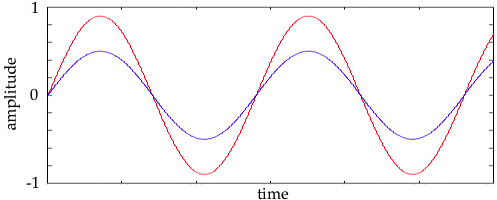
\includegraphics[width=.80\textwidth]{sprint1/samepitchdiffamp}
\caption{Two sound waves (represented as sine functions) with same frequency, but different amplitude.}
\label{fig:samepitchdiffamp}
\end{figure}

There is also a third characteristic, which is more abstract and not directly a physical attribute, namely, timbre.
Timbre is a composition of different sound waves (spectra), which makes up a specific sound (again, this is perceptual) and envelope (transients), which describe the different stages of a sound.

\subsection{Obtaining frequency}
Obtaining frequency is fairly simple, as it can read from a sound input interpreted as a wave (sine function).
However, some sounds are simpler than others in their composition of waves.
These simpler sounds could be considered ''cleaner'' than others, meaning they consist of only a single or very few waves, where it is easy to identify a primary amplitude and frequency.

Human speech, among other sounds, consists of multiple sound waves, each with varying amplitude and frequency.
In this case, it may be difficult to point out a single wave as the most important, and choose its frequency as the main frequency.
A comparison between frequency spectra can be seen in \cref{fig:frequency_spectra}.

\begin{figure}[h]
\centering
\begin{subfigure}[t]{.45\textwidth}
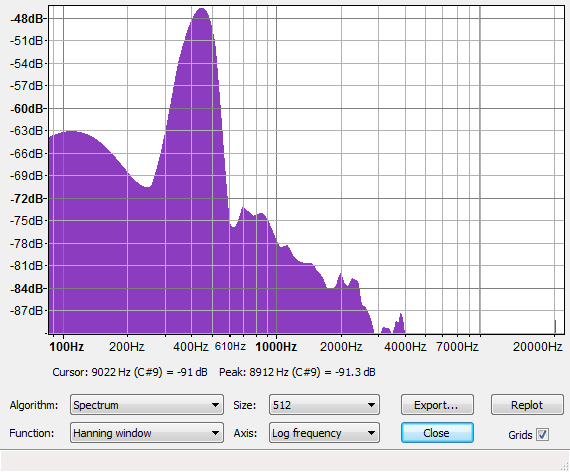
\includegraphics[width=\textwidth]{sprint1/spectrum_tonegenerator}
\caption{Frequency spectrum for a 440 Hz generated tone}
\end{subfigure}
\begin{subfigure}[t]{.45\textwidth}
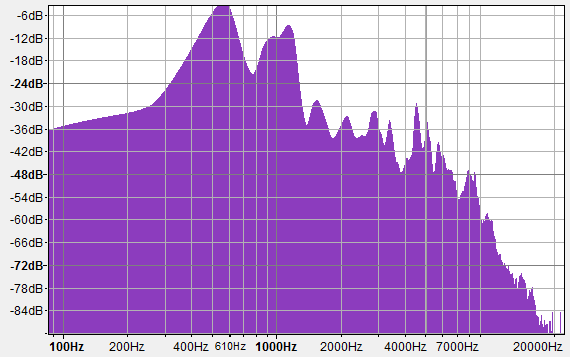
\includegraphics[width=\textwidth]{sprint1/spectrum_highpitchvoice}
\caption{Frequency spectrum for human voice input (in an attempt to reach high pitch)}
\end{subfigure}
\caption{Frequency analysis in Audacity}
\label{fig:frequency_spectra}
\end{figure}

\subsection{Using FFT}



\section{Design Evaluation}
The original goal of the first sprint was to refactor the Cars project. 
After using a few weeks reading and changing the code it turned out to be more complicated than initially assumed.
The changes we made was small but required extensive work because of the lack of structure in the project.
It was decided that a total redesign of the application would be the better option.
Instead of spending a lot of time trying to understand and modify the code, a redesign would not only take shorter time but would also result in a better design.

The following sections will summarize the problems that made the task of refactoring the cars project near impossible.
It seems that the authors of the code are not familiar with the OOP term inheritance.
Inheritance in OOP is when you have a class based on an other class.
This is useful for code reuse.

An example of good use of inheritance is if we have a class called \textit{Vehicle}.
Which e.g. has a method \textit{ChangeOwner} and a field \textit{RegistrationNumber}.
We can then make a specialisation of \textit{Vehicle} e.g. called \textit{Car} and \textit{Truck}.
These two new classes can now also use the method and field there is in \textit{Vehicle}.
This means the code gets reused, instead of having it in both \textit{Car} and \textit{Truck} we have it only in \textit{Vehicle}.

An example from 'Cars' is the class \textit{GameObject} which is an empty super class to the following classes:

\begin{tabular}{ c  c }
\parbox{\textwidth/2}{
\begin{itemize}
\item Barricade
\item Bump
\item Car
\end{itemize}} &
\parbox{\textwidth/2}{
\begin{itemize}
\item Cat
\item Garage
\item Rock
\end{itemize}
}
\end{tabular}
The classes shown above all have a \textit{draw} method which are identical.
This is a classic example on a method which should have been in the super class.
If it would have been in the super class all its derived classes could have used the method.
This would then be good code reuse.
This paragraph will contain the general problems with the methods in the project 'Cars' and their usability.
\\
Understanding a method is difficult when it is big and has different operations.
One should instead split them up to small methods, for instance an operation per method.
\\
An example of an operation could be to fill a whole array with a certain number.
The code for this would be a for-loop filling an array with the number.
Instead of having the code in the method, where you then will use it, it is better to create a method for that and call it.
This in general makes the maintenance and refactoring of the code easier, because the code then has a higher readability.
\\
The \textit{Run} method\cref{abe} from 'Cars' from the class \textit{RecorderThread} is a classic example on a method which should be smaller.
For the graphics in 'Cars' the authors have chosen to use OpenGL \cite{opengl}.
OpenGL is a tool for advanced graphics and it can be used for 3d graphics.
For a simple game like 'Cars' it is simply overkill.
As mentioned in the developer guide for Android \cite{android_opengl}.
The guide mentions that OpenGL should be used for advanced 3d graphics and if you need calculation power from the GPU.
Instead the guide suggest that the standard tools in the framework would be sufficient.
A problem throughout the code is that basic object oriented principles are not used or are not used properly. 
Classes do not have a clearly defined responsibility, and functionality is instead spread out on several classes. 
This breaks the concept of keeping high cohesion in object oriented design. 
Cohesion is a measure of how the responsibilities of a module are related. 
If the responsibilities are highly related, the module is said to have high cohesion.
An advantage of high cohesion is that it improves maintainability of the system, because changes in one module requires fewer changes in other modules. \stefan{source på cohesion (OOAD)?}

An example of low cohesion in the cars project is the \lstinline!Car! class(\cref{car_class}).
This class has the responsibility to draw itself, move itself according to pitch of the sound recorded by the microphone, calculate collisionboxes and determine if the car has collided with an obstacle and close the garage if the car has driven into the goal garage.

Another concept the existing code breaks is coupling.
Coupling is the number of  dependencies between modules.
It is desirable to keep this number as low as possible, known as having low coupling.
Low coupling has the advantage of making it easier to make changes in module, as they are not independent on each other.

When trying to read and understand the existing implementation of the control of the car by pitch, it turned out to be very hard.\stefan{possibly a reference to FFT analysis chapter}
Because the code responsible for handling the pitch is spread out on several classes, this relatively simple change becomes very complicated.
Another example is the responsibility for drawing objects which is on the individual object instead of using inheritance as described in \cref{sprint1_inheritance}. 
This makes it very hard to make consistent changes to the way objects are drawn.
\stefan{code examples?} 

\subsection{Redesigning Cars}
To best avoid ending in a situation similar to the above, it was deemed important that a framework was found on top of which the new game could be built.
Such a framework could define a \textit{proper} structure for game development, allowing the project group to focus solely on the game development without having to consider android.

\paragraph{Kilobolt}\label{kilobolt:description}
In \textit{''Beginning Android Games''}\cite{androidgames} an open source framework is suggested for game development.
The framework is presented and described on kilobolt.com\cite{kilobolt} using a simple example of a game.
The framework generalizes Java game development by defining a set of interfaces describing the structure of a game.

These interfaces are then implemented in an Android version specifying how the generalized framework should be executed on Android devices.
In the implementations presented on kilobolt.com there are some inconsistencies between the interfaces and Android implementations.
An example of this is that in some cases the Android implementation defines more methods than the interface.
Any such inconsistencies would have to be fixed if implementing for multiple platforms.
Simultaneously any future expansion of the framework would require all methods to be defined in both interfaces and Android implementations. 

Since the project for which the framework is used is Android-only, the generalized part of the framework was removed.

\subsubsection{The framework}
The following gives a description of the internals of the framework described above.
Not every class in the framework will be described as not all are essential to its functionality.

\paragraph{The Game Activity}
A game in the framework is implemented as an activity, allowing for simple interoperability with other Android components.
The game itself is primarily a shell, connecting the parts of the framework.
Actually implementing a game is done via screens.
A screen defines a \textit{state} in a game, drawing context specific graphics.
A game defines its initial screen, and screens are capable of replacing the active screen of a game.
Using this method, parts of a game can be implemented separate of the remaining game, resulting in higher cohesion.

\paragraph{Rendering}
In order to handle continuous updates of a game (frames) a separate thread is started, which performs these updates.
The thread uses a canvas for drawing, which is exposed only through a set of methods that draw on it.
Using this method rendering can be handled directly in screens without access to the canvas itself.
Ensuring that all drawing is done this way gives a low coupling of the rendering aspect of games.

Besides the canvas, the render-thread also uses a bitmap buffer which the canvas uses for drawing.
Whenever a new frame has been drawn, using the methods described above, the game activitys visual are updated, drawing the content of the buffer onto the view associated with the activity.
After the update a new frame-render is started.

As the rendering of frames is done continuously in a separate thread, there is no way to ensure a fixed framerate.
Instead the thread stores a timestamp whenever a frame has been rendered.
This is then later used to determine the time the has passed since the last frame.
This information can be used to properly update changes in a game, such as ensuring that a car moves at a constant speed.


\subsection{Solution}
\subsubsection{Change from Frequency to Volume}
Because of the problems obtaining the right frequency, explained in \cref{obtaining_frequency}, the idea was to change the control of the car to volume.
The idea was proposed to one of the stakeholders \textit{Tove Søby} (the speech therapist) so that there would not be worked on a solution which would not be used anyway.
The idea was accepted, see \cref{email_volume} for email correspondence.

Because of the decision to recreate the game from scratch, this sprint has been more like a pregame from SCRUM, and the actual product is therefore minimal.
The framework that was suggested in \cref{kilobolt:description} has been used to recreate a minimal working example of the game.
The result can be seen on \ref{product-sprint1}.

The car drives from left to right and is controlled by the volume of the player's voice. 
Loud sounds will make the car drive to its left while quiet sounds make it drive to its right.
Only sounds over a certain threshold makes the car move, meaning that no sound causes the car to drive straight forward.

The squares in the right side of the screen represent garages, and the color represents its state. 
A green garage is open, a yellow garage is closing while a red garage is closed.
It is possible to drive into a green garage which will then turn yellow for a short amount of time and then turning red.
If the car drives into a red garage it 'crashes', resetting its position to the starting position in left of the map vertically in the middle of the screen.

The purple squares represent obstacles that have to be avoided. 
If the car drives into one of these it 'crashes' and is being reset.


\begin{figure}
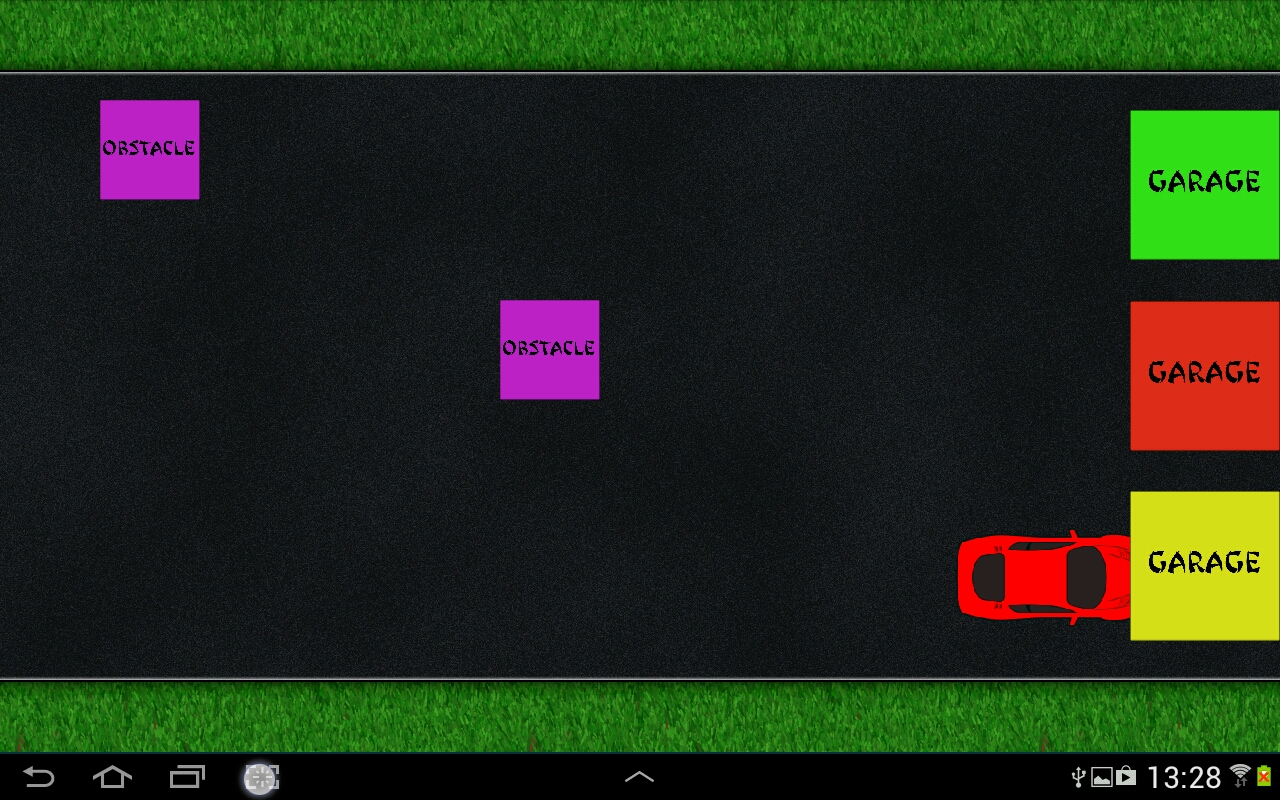
\includegraphics[width=\textwidth]{product}
\caption{The product after sprint 1}
\label{product-sprint1}
\end{figure}


This section contains an overview of the requirements and whether they have been fulfilled during this sprint.
If they are fulfilled it is explained how.
\begin{figure}[H]
\begin{tabular}{c|l|c|c}
\textbf{\#} & \textbf{Requirement} & \textbf{Solved} & \textbf{Link} \\
\hline
1. & \begin{tabular}[l]{@{}l@{}}The game must not be a side-scrolling game,\\because the citizen must be able to see the goal\end{tabular}
 & $\surd$ & \cref{sprint1:req1} \\
\hline
2. & \begin{tabular}[l]{@{}l@{}}The game must make it possible\\for the citizen to control a car\end{tabular}& $\surd$ & \cref{sprint1:req2} \\
\hline
3. & The game should contain stars as points & $\times$ & - \\
\hline
4. & The goal of the game is to reach a garage & $\surd$ & \cref{sprint1:req4} \\
\hline
5. & When the game is won an reward should be given & $\times$ & - \\
\hline
6. & \begin{tabular}[l]{@{}l@{}}It must be possible\\to save and load settings for a specific profile\end{tabular} & $\times$ & - \\
\hline
7. & It must be possible to calibrate the microphone & $\times$ & - \\
\hline
8. & \begin{tabular}[l]{@{}l@{}}It must be possible\\for the user to change the difficulty of the game\end{tabular} & $\times$ & - \\
\hline
\end{tabular}
\caption{Requirements fulfilled after sprint 1.}
\label{requirement_table_1}
\end{figure}
\paragraph{Requirement 1}\label{sprint1:req1}
Looking at \cref{product-sprint1} the game starts at the left side of the screen and ends at the right side of the screen, without any scrolling.
\paragraph{Requirement 2}\label{sprint1:req2}
It is possible to control the car with volume, making the car move up when the input volume is high and down when it is low.
The car stays at its position when there is no input.
For more detail can be found at \cref{sprint1:product}.
\paragraph{Requirement 4}\label{sprint1:req4}
Looking at \cref{product-sprint1} on the right side there are three boxes labelled 'garage', these represent the place where the graphics for the garages should be.
How they work is explained in \cref{sprint1:product}.
This section contain the assignments which should be considered looking at in the next sprint.

In the next sprint the focus should be on looking at the rest of the requirements, but especially improve and finish the following requirements.

\paragraph{Requirement 2}
The implementation of controlling the car right now only works using the microphone on the tablet used for the development process.
So in the next sprint there should be looked at a solution for this problem.
\paragraph{Requirement 4}
The boxes that are used as garages right now, should be replaced with some proper graphics.

\chapter{Sprint 2}

In the previous sprint, a new framework suggested for the 'Cars' app and the implementation of it was begun.
The main focus of this sprint is to continue this implementation, while getting some feedback from the stakeholders, to solve uncertainties regarding the old requirements.

The first part of this sprint chapter contains an interview with the stakeholders, from which new requirements were obtained.
The result is a new list of requirements, based on both the old requirements and the newly obtained.

Following the interview, the design and implementation of the new requirements can be seen.
This is done in an informal manner, explaining the overall idea, and results where appropriate.

The result of the sprint is a working application, which implements most of the requirements.
However, not all of them were fully implemented, and some not at all.
\newpage

% Introduction

\subsection{Purpose}

\subsection{Planning}

\subsection{Result}
Initially the requirements were the same as last sprint.
However, due to the interview carried out during the sprint, some new requirements were gathered, along with some of the old requirements being changed.

Here will be represented a new and complete list of requirements, as a merge between the initial requirements and the newly obtained.

\textbf{Note:} The following is based on \cref{sprint1:requirement_table_1}.
\Cref{sprint1:tab1:req2}  was vague so it was altered to \cref{sprint2:tab1:req2} on \cref{sprint2:requirement_table_1} so it now is more precise.
\Cref{sprint1:tab1:req3} was completely removed, as the focus should be on using the voice, not winning as such.
\Cref{sprint1:tab1:req8} was vague so it was split into several new requirements regarding difficulty from the interview.

\begin{tabularenumerate}
\begin{longtable}{c|l|c|c}
\textbf{\#} & \textbf{Requirement} & \textbf{Solved} & \textbf{Link} \\
\hline
\tabenum & \begin{tabular}[l]{@{}l@{}}The game must not be a side-scrolling game,\\because the citizen must be able to see the goal\end{tabular}
 & $\surd$ & \cref{sprint1:req1} \\
\hline
\tabenum \label{sprint2:tab1:req2} & \begin{tabular}[l]{@{}l@{}}The car is controlled in such a way,\\that the vertical position of the car is relative\\ to the current loudness of the player's voice.\end{tabular}& $\surd$ & \cref{sprint1:req2} \\
\hline
\tabenum & The goal of the game is to reach a garage & $\surd$ & \cref{sprint1:req4} \\
\hline
\tabenum & When the game is won an reward should be given & $\times$ & - \\
\hline
\tabenum & \begin{tabular}[l]{@{}l@{}}It must be possible\\to save and load settings for a specific profile\end{tabular} & $\times$ & - \\
\hline
\tabenum & It must be possible to calibrate the microphone & $\times$ & - \\
\hline
\tabenum & \begin{tabular}[l]{@{}l@{}}There is a digit between 0 and 10\\ displayed on the car as well as obstacles,\\ representing the loudness level,\\ based on its vertical position.\end{tabular} & $\times$ & - \\
\hline
\tabenum & \begin{tabular}[l]{@{}l@{}}Besides the scales from 0 to 10,\\ both speed and loudness have pictograms\\ illustrating some of the values on these scales.\end{tabular} & $\times$ & - \\
\hline
\tabenum & \begin{tabular}[l]{@{}l@{}}It should be possible to pause the game.\\ When the game is paused,\\ a loudness-barometer is displayed next to the car,\\ further visualizing the current loudness.\end{tabular} & $\times$ & - \\
\hline
\tabenum & \begin{tabular}[l]{@{}l@{}}Speed is alterable. The speed level\\ is represented as a digit between 0 and 10.\end{tabular} & $\times$ & - \\
\hline
\tabenum & \begin{tabular}[l]{@{}l@{}}The placement and number of obstacles\\ is alterable.\end{tabular} & $\times$ & - \\
\hline
\tabenum & \begin{tabular}[l]{@{}l@{}}The placement of obstacles should be\\ in such a way,\\ that it is possible to adapt it to both citizen\\ with tendency to speaking too loud\\ as well as those speaking too low.\end{tabular} & $\times$ & - \\
\hline
\tabenum & \begin{tabular}[l]{@{}l@{}}The graphics need to be simple,\\ as some citizens have a low attention span\\ and are easily distracted.\end{tabular} & $\times$ & - \\
\hline
\tabenum & \begin{tabular}[l]{@{}l@{}}It should be possible, in settings, to switch\\ between avoiding objects and picking objects up.\end{tabular} & $\times$ & - \\
\hline
\tabenum & \begin{tabular}[l]{@{}l@{}}When picking objects up, this is\\ linked to pictogram categories.\end{tabular} & $\times$ & - \\
\hline
\tabenum & \begin{tabular}[l]{@{}l@{}}It should be possible, in settings, to switch\\ between avoiding objects and picking objects up.\end{tabular} & $\times$ & - \\
\hline
\tabenum & \begin{tabular}[l]{@{}l@{}}It is important that the pickup/category\\ ''mode'' is optional, due to different capabilities\\ for each citizen.\end{tabular} & $\times$ & - \\
\hline
\caption{Requirements fulfilled after sprint 1.}
\label{sprint2:requirement_table_1}
\end{longtable}
\end{tabularenumerate}

\section{Design and Implementation}

\subsection{Sound and speed gauges}
The interview with the costumers (described in \cref{s2interview}) revealed that they use a gauge system to illustrate speeds and volume levels at the institution. 
The gauges used are pictured in \cref{gauges}.
Each gauge is from 0 to 10, and some of the levels have a pictogram associated.

\begin{figure}[h]
	\centering
        \begin{subfigure}[b]{0.5\textwidth}
                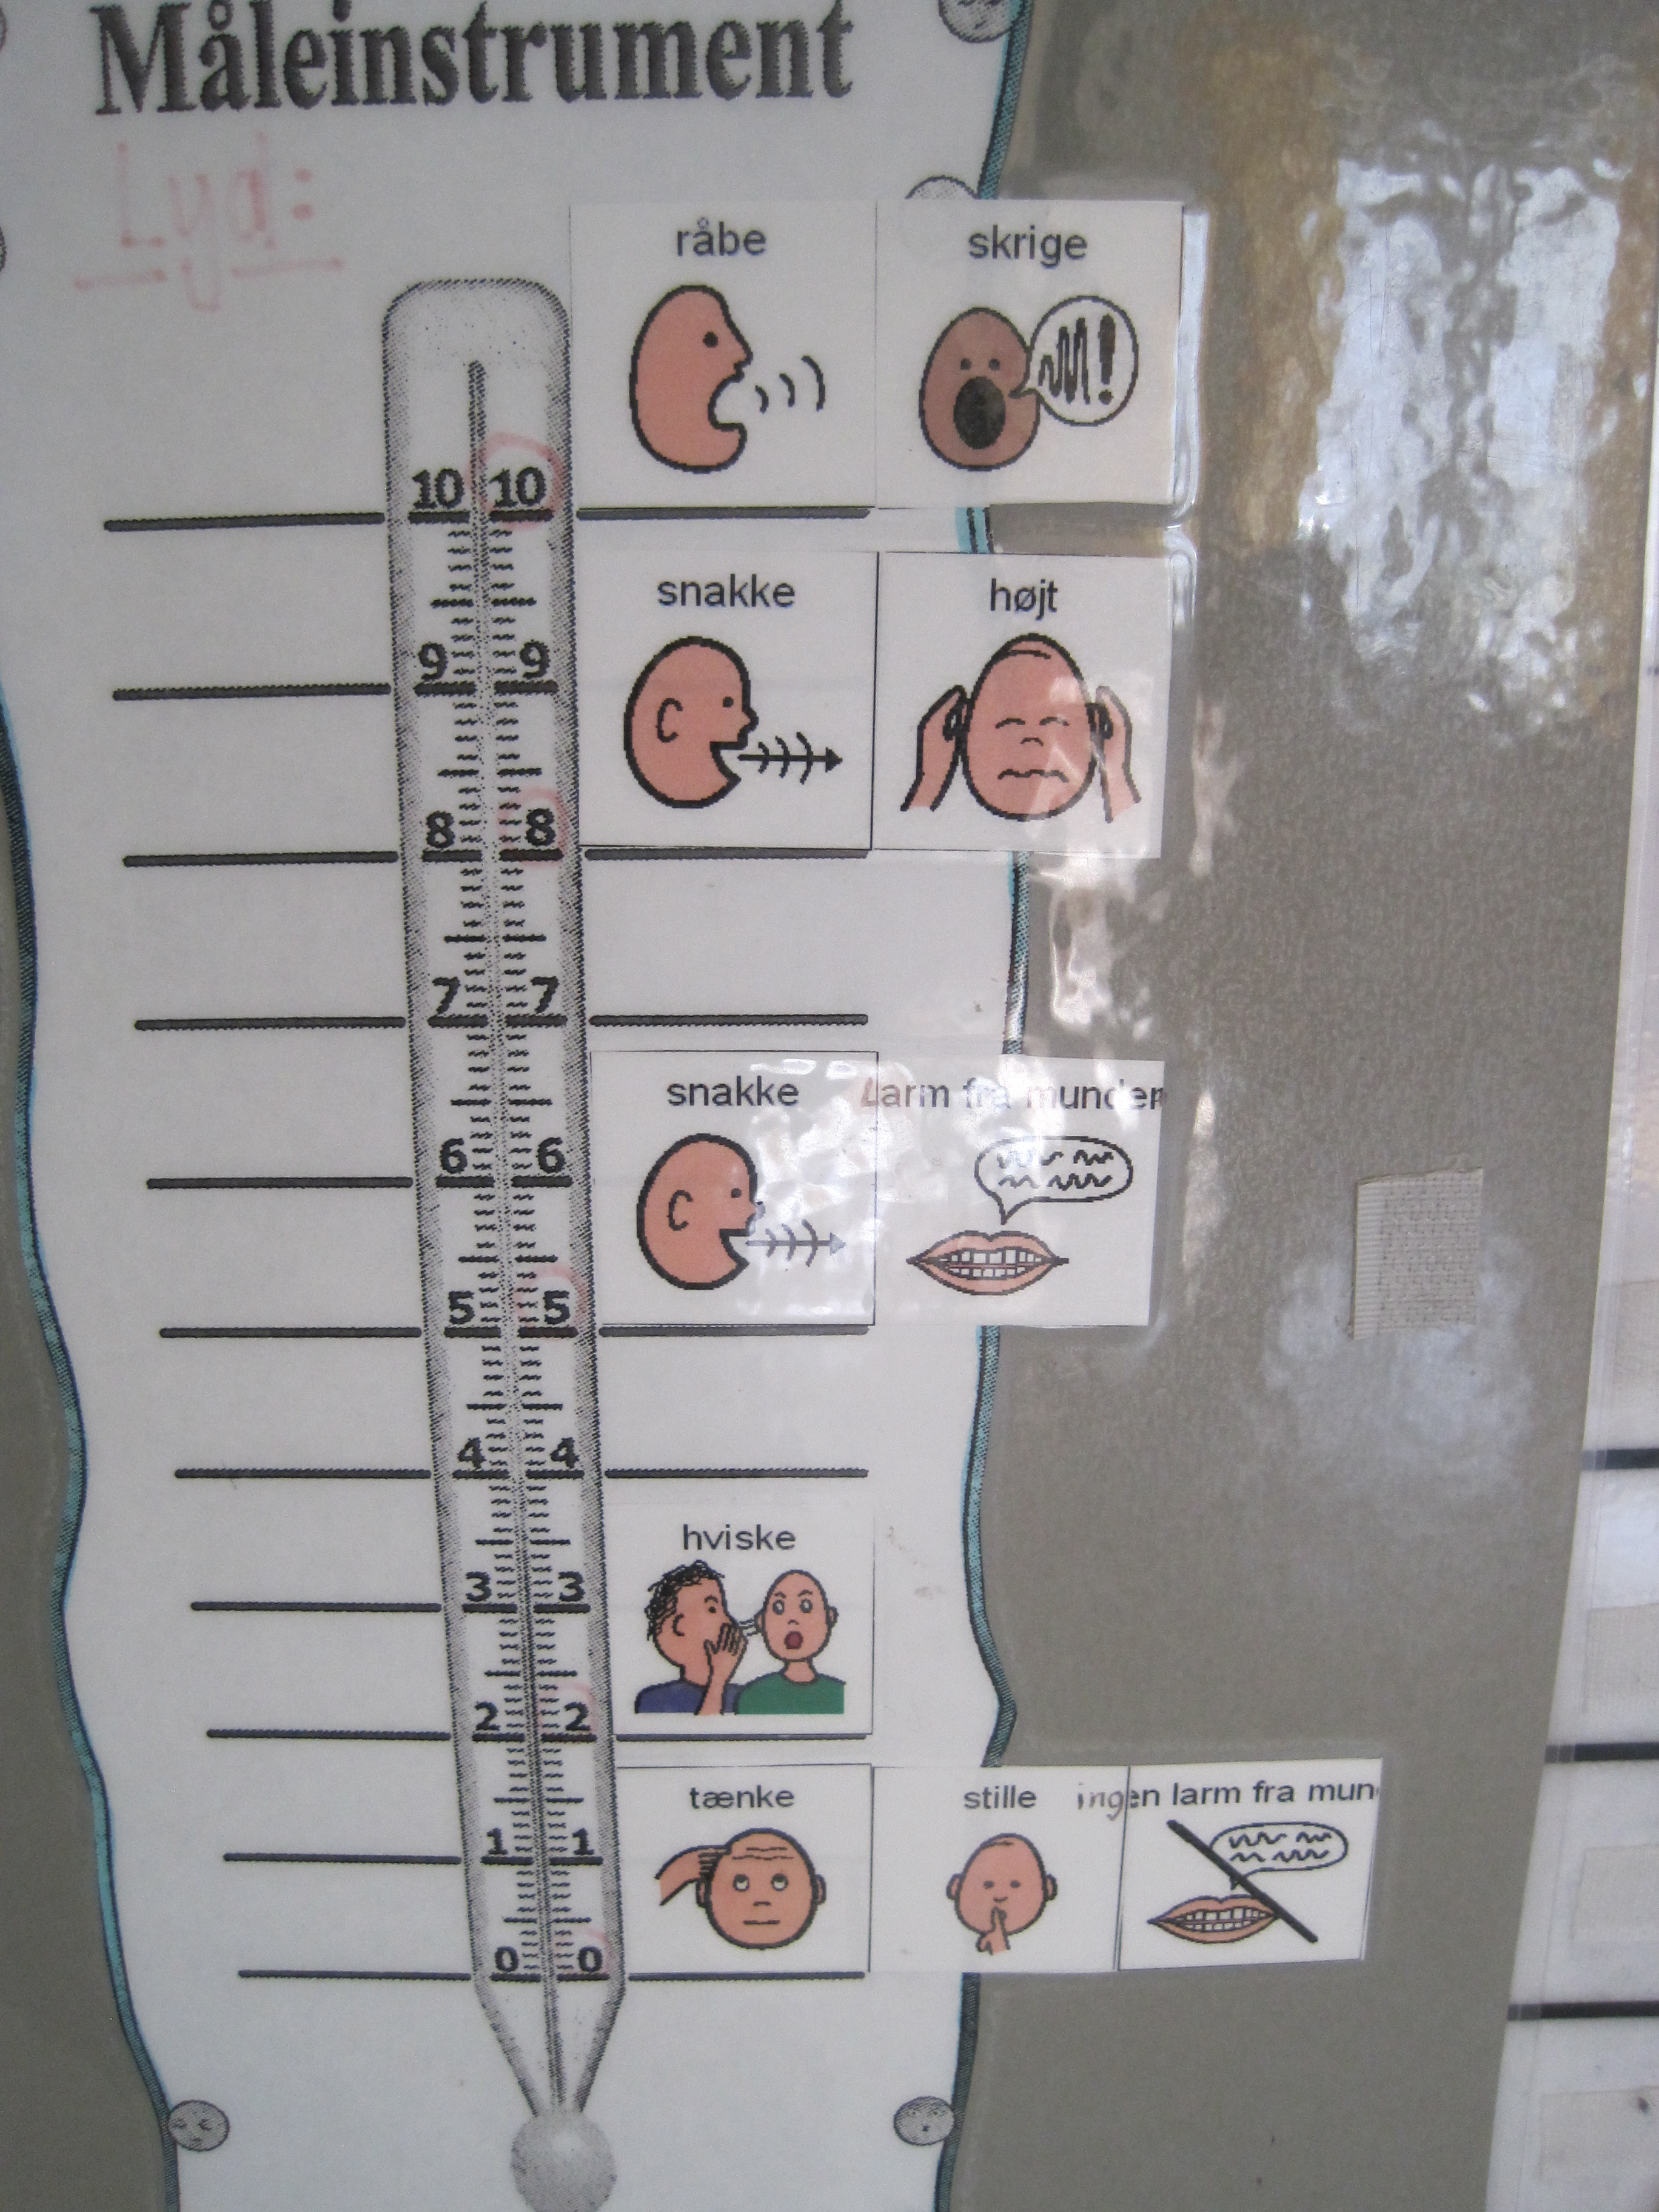
\includegraphics[width=\textwidth]{sound}
                \caption{The sound gauge}
                \label{soundgauge}
        \end{subfigure}%
        ~
        \begin{subfigure}[b]{0.5\textwidth}
                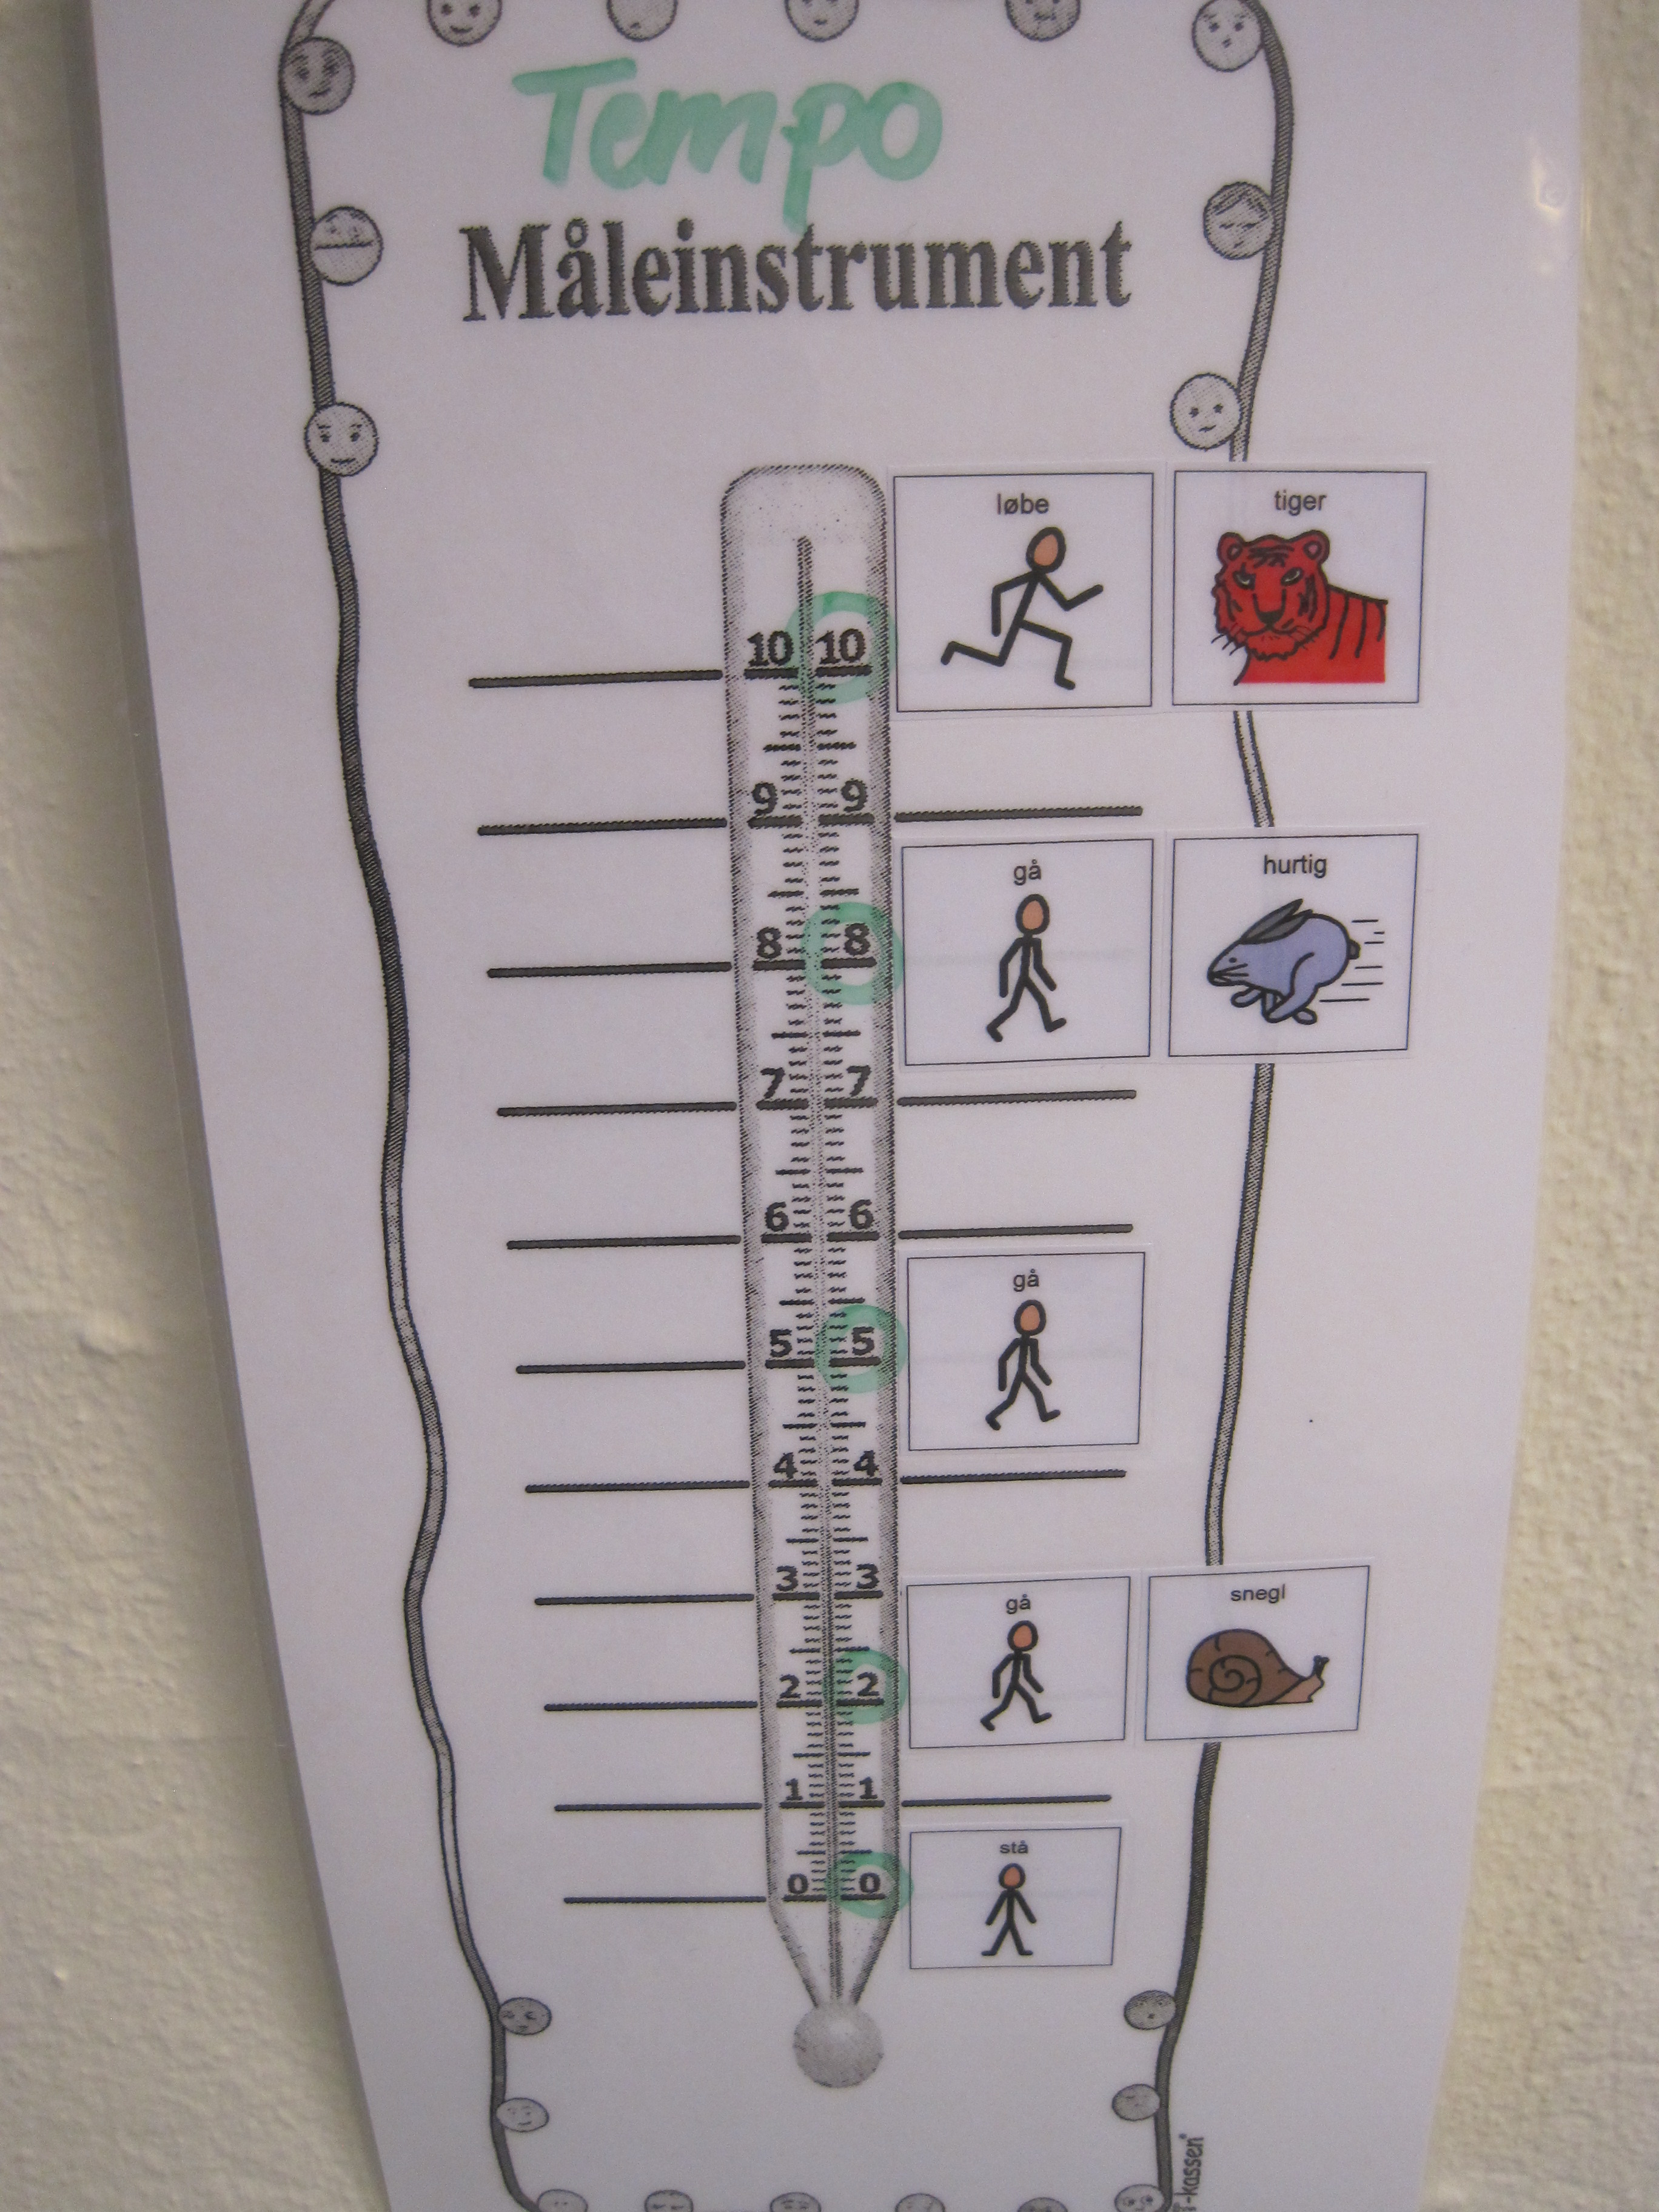
\includegraphics[width=\textwidth]{speed}
                \caption{The speed gauge}
                \label{speedgauge}
        \end{subfigure}
        \caption{The gauges used at 'Birken'}\label{fig:animals}
        \label{gauges}
\end{figure}

Several requirements (described in \cref{s2requirements}) is about incorporating these gauges in the game.
The requirements concerning the gauges are as follows:

\begin{enumerate}
\setcounter{enumi}{6}
\item \label{visualnumber} There is a digit between 0 and 10 displayed on the car as well as obstacles, representing the loudness level, based on its vertical position. 
\item \label{pictogram} Besides the scales from 0 to 10, both speed and loudness have pictograms illustrating some of the values on these scales.
\item \label{pause} It should be possible to pause the game. When the game is paused, a loudness-barometer is displayed next to the car, further visualizing the current loudness.
\item \label{speeditem} Speed is alterable. The speed level is represented as a digit between 0 and 10.
\end{enumerate}


\paragraph{Requirement \ref{visualnumber}} is met by drawing the number corresponding to the position of the object on the gauge. 
This can be seen on \cref{pausedstate}.

\paragraph{Requirement \ref{pictogram}} was not fulfilled in this sprint.


\paragraph{Requirement \ref{pause}} is partially fulfilled.
The pause functionality is achieved by having a pause button in the upper left corner. 
When the game is paused the game is faded out, and a representation of the gauge is placed left of the car so it is possible to see the full scale in the game area.
This can be seen on \cref{pause}.
This placeholder scale is to be replaced with a gauge similar to the one seen on \cref{soundgauge}.

The fulfilment of these two requirements can be seen on \cref{pausedstate}.

\begin{figure}
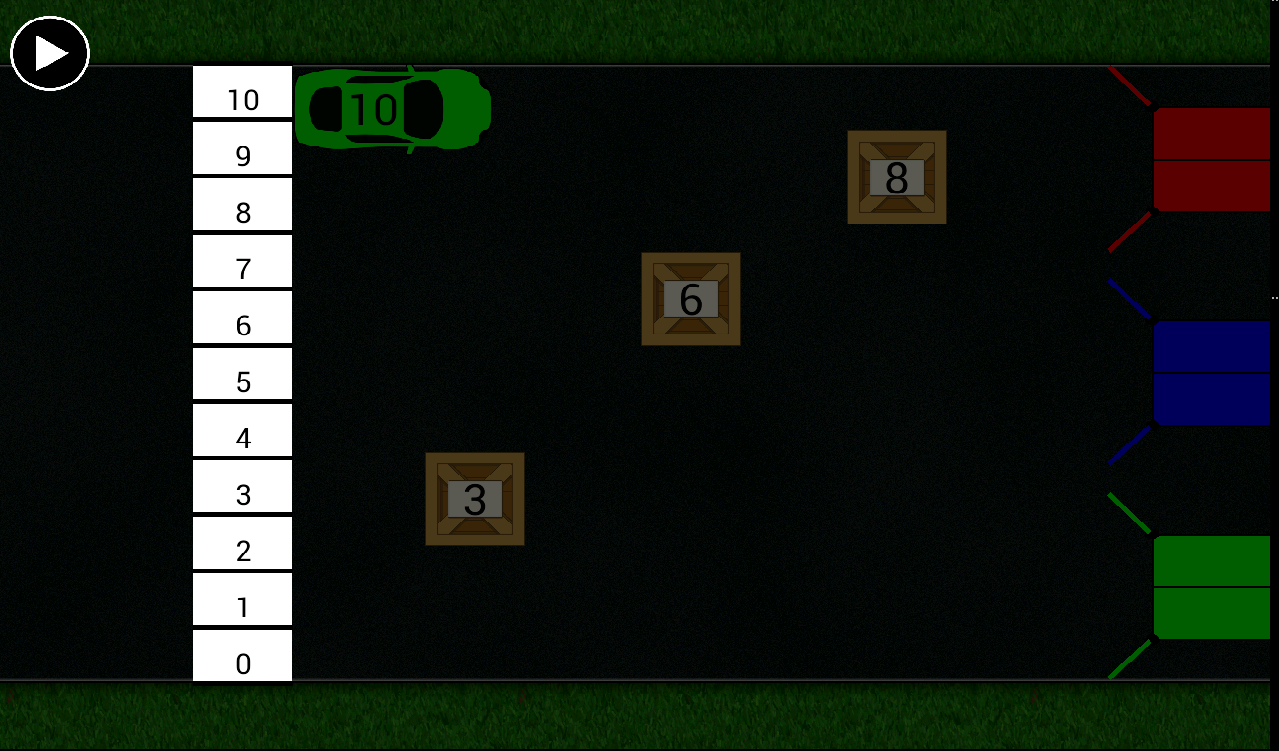
\includegraphics[width=\textwidth]{pause}	
\caption{The game in a paused state. The game is seen in the background and a sound gauge is shown left of the car}
\label{pausedstate}
\end{figure}


\paragraph{Requirement \ref{speeditem}} was only partially fulfilled in this sprint, by making the speed alterable. 
The gauges and pictograms are not yet visible on the settings module, which can be seen on \cref{speedsettings}.
The shown number is the value of speed used internally.
The speed is altered by pressing in the left or right side, decreasing or increasing the speed respectively.
These 'invisible' buttons are to be changed to pictograms from the gauge on \cref{speedgauge}.

\begin{figure}

\includegraphics[width=\textwidth]{speedSettings}
\caption{The temporary implementation of alteration of the speed}
\label{speedsettings}
\end{figure}




\subsection{Screen overlays}
At certain stages of the game, we need to display overlays, containing important information and/or buttons for navigation.

The game screen contains the following overlays:

\begin{itemize}
\item Starting,
\item Paused,
\item Crashed, and
\item Won.
\end{itemize}

All of the screens can be seen in \cref{sprint2:overlays:fig}.

\paragraph{Starting Overlay} is displayed when a new game is started (from either the main menu or the Win Overlay).
It is a short countdown, enabling the player to get ready, as opposed to starting the game straight away, or simply waiting without any feedback for the player.
It is a 3 second countdown (3.. 2.. 1.. Go), as can be seen in \cref{sprint2:overlays:fig:starting}.

\paragraph{Paused overlay} is linked to requirement 9, which states: \textit{It should be possible to pause the game. When the game is paused, a loudness-barometer is displayed next to the car, further visualizing the current loudness.}
At all times when in the game screen, a pause button is visible in the top left corner.
When pressed, the game is paused (the car stops moving) and the loudness gauge is displayed (see \cref{sprint2:overlays:fig:paused}).
\subsection{Graphics}
According to \cref{sprint2:tab1:req13} in \cref{sprint2:requirement_table_1}, the graphics must be kept simple.
To accommodate this both the background and the objects have been kept simple and two dimensional.
The graphics used in the game can be seen on \cref{pausedstate}.
The background consists of a road which is a grey texture, and there is a border of grass in the top and the bottom of the screen, consisting of a green texture.

\begin{figure}[h]
\begin{subfigure}{0.5\textwidth}
\centering

\includegraphics{car}
\caption{The car}
\label{car}
\end{subfigure}
~
\begin{subfigure}{0.5\textwidth}
\centering
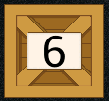
\includegraphics{obstacle}
\caption{An obstacle}
\label{obstacle}
\end{subfigure}

\begin{subfigure}{\textwidth}
\centering
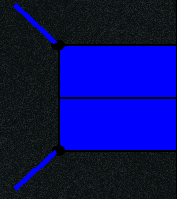
\includegraphics{garage}
\caption{One of the garages}
\label{garage}
\end{subfigure}
\caption{The graphics used in the game}
\label{graphicszoom}
\end{figure}

The individual objects can be seen on \cref{graphicszoom}.
The objects are chosen so they are simple and yet recognizable.
\subsection{Control of the car}
At the interview the costumers expressed that they needed to change how the car was controlled.
They wanted the car to reflect the current sound level of the speech recorded by the microphone.
This is expressed in requirement \ref{carcontrolReq} which is as follows:
\begin{enumerate}
\setcounter{enumi}{5}
\item The car is controlled in such a way, that the vertical position of the car is relative to the current loudness of the player's voice.
\end{enumerate}

This has been implemented in the game by mapping the values recorded by the microphone to a range that corresponds to the height of the screen.
This mapping is shown on \cref{mapping}.
The microphone records sounds and outputs values between 0 and some max value, shown as 1000 for simplicity.
When calibrating the microphone two values are defined, the minimum value reflecting background noise caught by the microphone, and the maximum value determined by the sound level of the player's shouting.
These two values are mapped to values between 0 and the size of the screen, in the example 800.

The returned value is the position on the screen where the car needs to drive towards at the current sound level.

\begin{figure}
\centering
\begin{tikzpicture}
%vertical scales
\draw (0,0) -- (0,3); 
\draw (3,0) -- (3,2);

\node [below] at (0,-0.5){microphone input};
\node [below] at (3,-0.75){screen position};

%  endpoints with labels
\draw (-0.1,0) -- (0.1,0); 
\node [below] at (0,0){0};

\draw (-0.1,3) -- (0.1,3);
\node [above] at (0,3){1000};

\draw (2.9,0) -- (3.1,0); 
\node [below] at (3,0){0};

\draw (2.9,2) -- (3.1,2);
\node [above] at (3,2){800};

%min and max labels 
\draw (-0.1,1) -- (0.1,1);
\node [left] at (0,1){min};

\draw (-0.1,2) -- (0.1,2);
\node [left] at (0,2){max};

% mapping lines
\draw [dashed, blue](0,2) -- (3,2);
\draw [dashed, blue](0,1) -- (3,0);
\end{tikzpicture}
\caption{The mapping from microphone input to position on the screen}
\label{mapping}
\end{figure}

\stefan{pseudoalgoritme?}


\subsection{Map Editor}
The map editor has been developed due to \cref{sprint2:tab1:req11} and \cref{sprint2:tab1:req12} in \cref{sprint2:requirement_table_1}.
The map editor makes it possible for the user to make a map that fits to the citizen's needs.
A screenshot can be seen on \cref{fig:sprint2:map_editor}, where there are added two obstacles.
The map editor is a screen of the game with only garages.
Users are able to add an obstacle by touching the screen - and the obstacle will be placed there.
Users can remove an obstacle by touching it.

\begin{figure}[h]
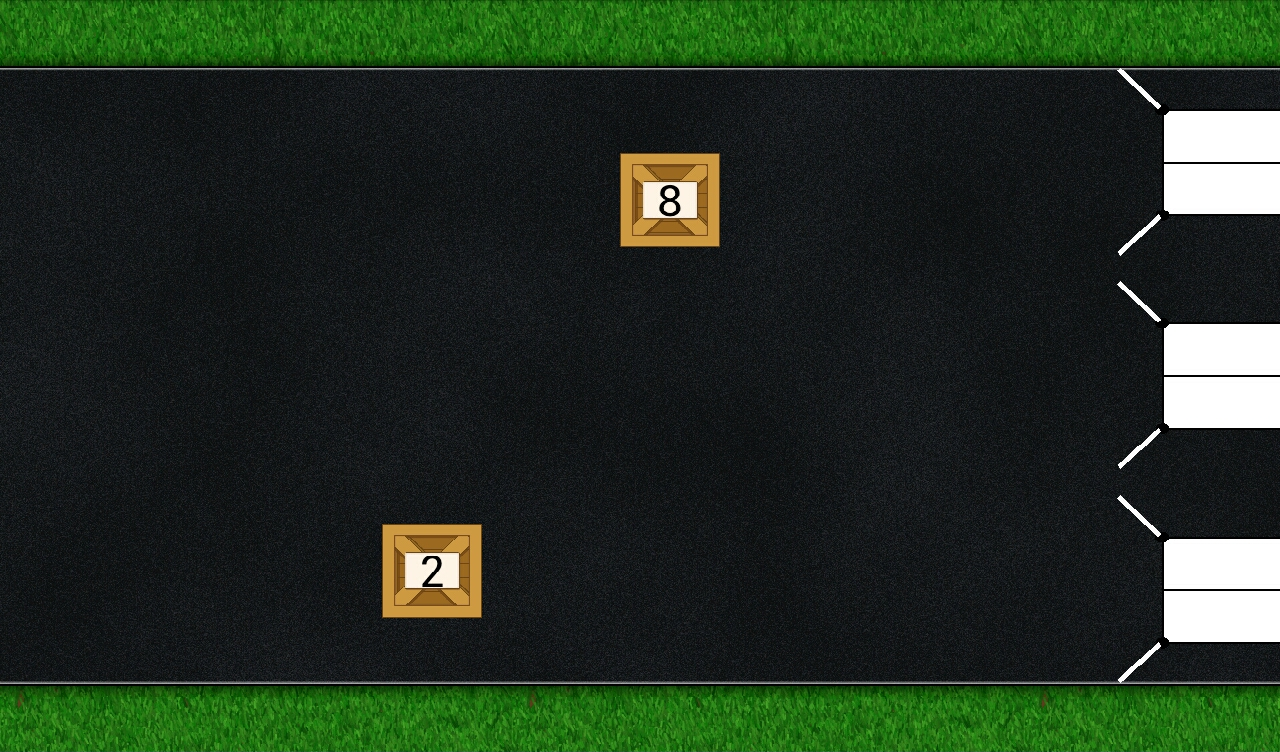
\includegraphics[width=\linewidth]{sprint2/map_editor}
\caption{The map editor, which makes it possible to customize the obstacle placement.}
\label{fig:sprint2:map_editor}
\end{figure}
 

\subsection{Settings}

The customization (settings) of the game is linked to requirements \ref{sprint2:requirements:profile}, \ref{sprint2:requirements:calibrate}, \ref{sprint2:tab1:req10}, \ref{sprint2:requirements:avoidorpickup}, and \ref{sprint2:requirements:categorymode} (see \cref{sprint2:requirement_table_1}).

\paragraph{Note:} Requirements \ref{sprint2:tab1:req11} and \ref{sprint2:tab1:req12} are also linked to settings, but this is handled seperately by the ''map editor'', which is explained in \cref{sprint2:map_editor}.\\

\noindent
The settings activity handles three things; Altering the speed of the car, Changing the colors of the garages, and Calibrating the microphone.
A screenshot of the settings activity can be seen in \cref{sprint2:settings:fig}.
\begin{center}
\begin{figure}
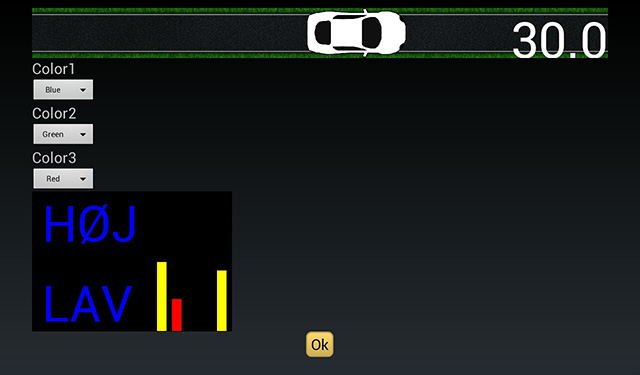
\includegraphics[width=\textwidth]{settings}
\caption{The settings activity}
\label{sprint2:settings:fig}
\end{figure}
\end{center}
\paragraph{Speed} is changed by tapping the ends of a small fragment of the game, displaying only one lane and the moving car.
By tapping the left end, the speed is decreased and by tapping the right, it is increased.
Whenever a change to speed is made, it is immediately visible in the game fragment.
The ability to alter the speed is directly related to requirement \ref{sprint2:tab1:req10}.

\paragraph{Color} is as of now changed by picking a color from a dropdown box.
This is not stated as a requirement, but is a feature that was implemented by the previous Cars project.

\paragraph{Microphone Calibration} is done in a small game fragment, as can be seen in the bottom of the settings screenshot.
This is in regards to requirement \ref{sprint2:requirements:calibrate}.
The way it is done atm, is when holding either 'H\o j' (high) or 'Lav' (low) down, during this time the microphone records and when they are released the average of all the recordings during the time are averaged and set as the appropriate threshold value.


\paragraph{Requirement \ref{sprint2:requirements:profile}} regarding loading and saving settings to a profile is not yet implemented.

\paragraph{Requirements \ref{sprint2:requirements:avoidorpickup} and \ref{sprint2:requirements:categorymode}} regarding picking up category pictograms is not yet implemented either.

\begin{tabularenumerate}
\begin{longtable}{c|l|c|c}
\textbf{\#} & \textbf{Requirement} & \textbf{Solved} & \textbf{Link} \\
\hline
\tabenum & \begin{tabular}[l]{@{}l@{}}The game must not be a side-scrolling game,\\because the citizen must be able to see the goal\end{tabular}
 & $\surd$ & \cref{sprint1:req1} \\
\hline
\tabenum \label{sprint2:tab2:req2} & \begin{tabular}[l]{@{}l@{}}The car is controlled in such a way,\\that the vertical position of the car is relative\\ to the current loudness of the player's voice.\end{tabular}& $\surd$ & \cref{sprint2:car_control} \\
\hline
\tabenum & The goal of the game is to reach a garage & $\surd$ & \cref{sprint1:req4} \\
\hline
\tabenum \label{sprint2:tab2:req4} & When the game is won an reward should be given & $\surd$ & \cref{sprint2:won} \\
\hline
\tabenum & \begin{tabular}[l]{@{}l@{}}It must be possible\\to save and load settings for a specific profile\end{tabular} & $\times$ & - \\
\hline
\tabenum & It must be possible to calibrate the microphone & $\times$ & - \\
\hline
\tabenum \label{sprint2:tab2:req7} & \begin{tabular}[l]{@{}l@{}}There is a digit between 0 and 10\\ displayed on the car as well as obstacles,\\ representing the loudness level,\\ based on its vertical position.\end{tabular} & $\surd$ & \cref{sprint2:gauges} \\
\hline
\tabenum & \begin{tabular}[l]{@{}l@{}}Besides the scales from 0 to 10,\\ both speed and loudness have pictograms\\ illustrating some of the values on these scales.\end{tabular} & $\times$ & - \\
\hline
\tabenum \label{sprint2:tab2:req9} & \begin{tabular}[l]{@{}l@{}}It should be possible to pause the game.\\ When the game is paused,\\ a loudness-barometer is displayed next to the car,\\ further visualizing the current loudness.\end{tabular} & $\surd$ & \cref{sprint2:paused} \\
\hline
\tabenum & \begin{tabular}[l]{@{}l@{}}Speed is alterable. The speed level\\ is represented as a digit between 0 and 10.\end{tabular} & $\times$ & - \\
\hline
\tabenum \label{sprint2:tab2:req11} & \begin{tabular}[l]{@{}l@{}}The placement and number of obstacles\\ is alterable.\end{tabular} & $\surd$ & \cref{sprint2:map_editor} \\
\hline
\tabenum \label{sprint2:tab2:req12} & \begin{tabular}[l]{@{}l@{}}The placement of obstacles should be\\ in such a way,\\ that it is possible to adapt it to both citizen\\ with tendency to speaking too loud\\ as well as those speaking too low.\end{tabular} & $\surd$ & \cref{sprint2:map_editor} \\
\hline
\tabenum \label{sprint2:tab2:req13} & \begin{tabular}[l]{@{}l@{}}The graphics need to be simple,\\ as some citizens have a low attention span\\ and are easily distracted.\end{tabular} & $\surd$ & \cref{sprint2:graphics} \\
\hline
\tabenum & \begin{tabular}[l]{@{}l@{}}It should be possible, in settings, to switch\\ between avoiding objects and picking objects up.\end{tabular} & $\times$ & - \\
\hline
\tabenum & \begin{tabular}[l]{@{}l@{}}When picking objects up, this is\\ linked to pictogram categories.\end{tabular} & $\times$ & - \\
\hline
\tabenum & \begin{tabular}[l]{@{}l@{}}It should be possible, in settings, to switch\\ between avoiding objects and picking objects up.\end{tabular} & $\times$ & - \\
\hline
\tabenum & \begin{tabular}[l]{@{}l@{}}It is important that the pickup/category\\ ''mode'' is optional, due to different capabilities\\ for each citizen.\end{tabular} & $\times$ & - \\
\hline
\caption{Requirements fulfilled after sprint 1.}
\label{sprint2:requirement_table_2}
\end{longtable}
\end{tabularenumerate}
\section{Future Works}
This section contain the assignments which should be considered looking at in the next sprint.
In the next sprint the focus should be on looking at the rest of the requirements, but especially improve and finish the settings and the control of the car.
The specifics of these assignments will be discussed in the following.

\subsection{Settings}
The main topic which has to be improved are the settings.
The layout, \cref{sprint2:settings:fig}, has to be modified so that it is clear which settings group together and what it is the user is able to change.
The three colours chosen for the garage should also be changed so the user is able to pick an arbitrary colour.
The microphone calibration setting also has to get changed to some more suitable layout.

\subsection{Control of the car}\label{sprint2:eval:control_car}
The control of the car does still not function properly with the calibration in the settings.
It seems that when the car was calibrated it does not work properly in the game, but when using hardcoded values the game works quite okay.
The problem therefore seems to be the calibration in the settings.


\chapter{Sprint 3}
In the previous sprint it was suggested to work on the settings and the control of the car.
So the main focus for this sprint was to work on these two.

In the settings activity there was some major changes in the way the speed is set.
A speed gauge was added, and the desired speed is set by pressing at the corresponding position on this gauge.

The selection of colors was changed to display a box filled with the selected color, and this box can be pressed to open up the color selector.


At last the application was hooked up to the common database so that the users settings are saved and synchronized.

\mikael{introduktion skal opdateres så den passer med det ændret indhold}
\section{Settings}\label{sprint3:settings}

Since the requirements hasn't changed at all since last sprint, the ones regarding settings remain the same.
During this sprint the following requirements were handled; \ref{sprint2_database_req}, \ref{sprint2:req:calibrate}, \ref{sprint2:req:picto_gauge}, and \ref{sprint2:req:speed} (see \cref{sprint2:requirement_table_2}).

\paragraph{Note:} Requirement \ref{sprint2_database_req}, regarding saving and loading settings, is described in \ref{sprint3:database}.\\

\noindent
The settings activity still handles the same three things as previously; speed of the car, garage colors, and calibration of the microphone.
The way in which the speed is altered was changed, along with how the garage colors are chosen.
Calibration of the microphone was not changed, as no proper solution was found this sprint.
A screenshot of the settings activity can be seen in \cref{sprint3:settings:screenshot}.

\begin{figure}
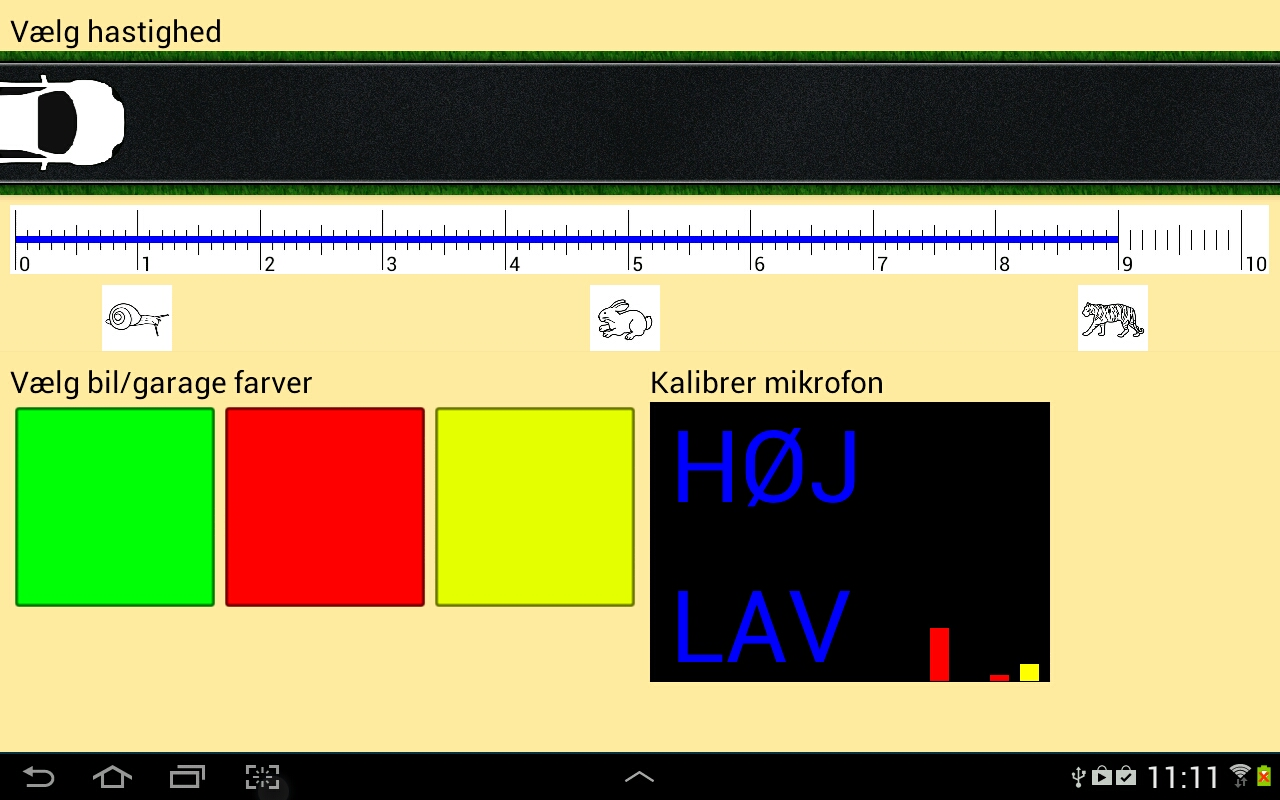
\includegraphics[width=\textwidth]{sprint3/settings_screenshot}
\caption{Screenshot of the Settings activity}
\label{sprint3:settings:screenshot}
\end{figure}

\paragraph{Altering of Speed} was changed according to requirements \ref{sprint2:req:picto_gauge} and \ref{sprint2:req:speed}.
The speed is set by either pressing the gauge, changing the position of the gauge-bar, which indicates the currently set speed.
Alternatively the pictograms (currently three; snail, rabbit, and tiger) can be pressed, moving the gauge-bar and setting the speed appropriately.

\paragraph{Choosing car/garage colors} is now depicted as a colored box, where the box's color is corresponding to the selected car/garage color.
A color can then be changed by pressing one of these boxes and choosing a new one from a standard color-picker.
\section{Connection to the database}
\label{sprint3:database}
In order to save the settings of the current user and make it available on all tablets with the Giraf applications installed, it is necessary to connect to the database.
This requirement in stated in \cref{sprint2_database_req} in \cref{sprint2:requirement_table_2}.
For this purpose the \lstinline!DatabaseHelper! class was created.
This class contains methods for saving and loading settings from the database. 

When the Cars application is launched, a \lstinline!child_id! and a \lstinline!guardian_id! is passed to the application. 
This identification number identifies the child that is currently using the tablet.
This identification number is used to load the correct settings when they are needed, which is in the game, in the settings window and in the mapeditor.
The settings are saved to the database when either the settings window or the mapeditor is closed.
\section{Stabilizing the car}
\mikkel{Jeg ved ikke hvor det her skal placeres...}
The cars' vertical motion is determined by voice input.
Using the volume recorded by the microphone, a value in the interval $[0-1]$ is calculated, where 0 represents silence and 1 represents \textit{maximum} volume.
The value is then mapped linearly to a vertical position in the game.
After this calculation is completed and a final value is determined, the car must be moved.

\paragraph{Positioning the car}
Given a vertical position where the car \textit{should} be placed, the car could simple be moved to its destination on each frame update.
This is the simplest solution as it requires no additional translation of the position input.
Let $m_f \in [0 \dots 1]$ represent the translated measurement at frame $f$ and $c_f \in [0 \dots 1]$ represent the position of the car at frame $f$.

\begin{center}
We then have that $c_f = m_f$.
\end{center}

There is however a problem with this approach.
The input from the microphone will sometimes yield spikes\footnote{
In this context \textit{spikes} refers to any deviation in the measured amplitude.
This includes any white noise recorded by the microphone.} in terms of the amplitude.
The reason for these spikes has yet to be determined.
The effect however is quite clear.
The car \textit{jumps} whenever such a spike is recorded, rendering it difficult for the user to map the voice level to the cars position.

To resolve this problem, various methods for \textit{moving} the car were attempted.
In the following sections these methods will be discussed.

\subsection{Linear motion}\label{stability:linear}
Instead of moving the car directly to its target location, it could be moved there \textit{over time}.
This naturally introduces a concept of speed, as to define how much time is required to move the car.
Let $s$ denote the vertical speed of the car and $t_f$ the time at frame $f$.
We then introduce the variable $\lambda_f = t_f - t_{f-1}$, representing the time difference between two frames.
With this, the position of the car can be represented as: $$c_f = \left\{ 
  \begin{array}{l l}
    c_{f-1} + s \cdot \lambda_f & \quad \text{if $c_{f-1} < m_f$}\\
    c_{f-1} - s \cdot \lambda_f & \quad \text{otherwise}
  \end{array} \right.$$

Using this approach the car no longer performs vertical leaps and will steadily move towards its current target.

The aforementioned spikes in volume are still present, as the same input is used.
This means that while the car is moving downwards it might move upwards for a few frames before continuing its ''correct'' motion.
The result is a car that jitters while it moves.

It is clear that while this approach fixes the issue of the car jumping from one position to another, there is still no clear mapping between the cars motion and the voice input.

\subsection{Averaging the measurements}\label{stability:average}
To reduce the effect of the spikes the average of the last $x$ measurements could be used instead of the actual measurements.
This would greatly reduce the jitter described above, as a single ''up'' measurement is outweighed by $x-1$ ''down'' measurements (assuming the deviations are similar).
Naturally we would still like the benefits of the linear motion (section \ref{stability:linear}) to keep the car from \textit{''jumping''}.
Let $m^{'}_{f}$ denote the average of the last $x$ measurements:
$$m^{'}_{f} = \frac{m_f + m_{f-1} + \dots + m_{f-x+2} + m_{f-x+1}}{x}$$
We can now define the cars position using this average:
$$c_f = \left\{ 
  \begin{array}{l l}
    c_{f-1} + s \cdot \lambda_f & \quad \text{if $c_{f-1} < m^{'}_{f}$}\\
    c_{f-1} - s \cdot \lambda_f & \quad \text{otherwise}
  \end{array} \right.$$

This method handles the spikes better than the strictly linear method.
For larger spikes a bigger value of $x$ is required to compensate.
The result of this is a significant delay in the effect of raising the volume of ones voice.

\subsection{Acceleration and deceleration}\label{stability:acceleration}
Another approach to managing the cars position is by having the car accelerate and decelerate when moving vertically.
Spikes in volume would then be met with a deceleration in speed.
But as they are often quite short-lived the car would quickly accelerate again.
Thus the spikes problem is solvable using this methodology.
Meanwhile the delay associated with averaging the measurements (section \ref{stability:average}) does not occur as the car always accelerates or decelerates depending on the actual input.
Using this method for moving the car can be defined as below:
$$c_f = c_{f-1} + s_f \cdot \lambda_x$$
Where $s_f$ refers to the cars vertical speed at frame $f$.
We are then left to define $s_f$ in a way that involves acceleration and deceleration using $s_{f-1}$ and $\lambda_x$ as the only variables.
For this purpose a function $speed$ is introduced, yielding the following equation:
$$c_f = c_{f-1} + \text{speed}(s_{f-1}, \lambda_x) \cdot \lambda_x$$\mikkel{Skal vi inkludere den egentlige funktion der definerer accelerationen? Jeg har det muligvis liggende i noget gammelt backup :P}
We will not explore the actual function that defines the acceleration of the car in the context of the cars vertical motion as it is the methodology of how the car is moved that is of interest.
Allowing the car to accelerate solves the problem caused by spikes in the voice input and gives direct feedback for the user.
Thusly this is the chosen solution to control the car.
\section{GUI Components}\label{sprint3:gui}
During this sprint we also implemented the use of the shared GUI components, through the library \lstinline|giraf-components|.
We used two components; \lstinline|GButton| and \lstinline|GColorPicker|.
Additionally we used the standard background color, provided by the library.
The button and colorpicker components can be seen in \cref{sprint3:guicomponents:fig}.

\begin{figure}[h]
\begin{subfigure}{0.49\textwidth}
\centering
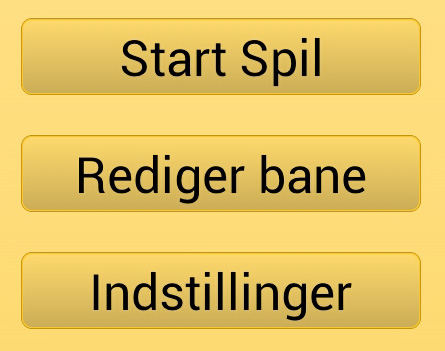
\includegraphics[width=0.49\textwidth]{sprint3/gbutton}
\caption{The \lstinline|GButton|s in Cars main Activity}
\label{sprint3:guicomponents:fig:gbutton}
\end{subfigure}
~
\begin{subfigure}{0.49\textwidth}
\centering
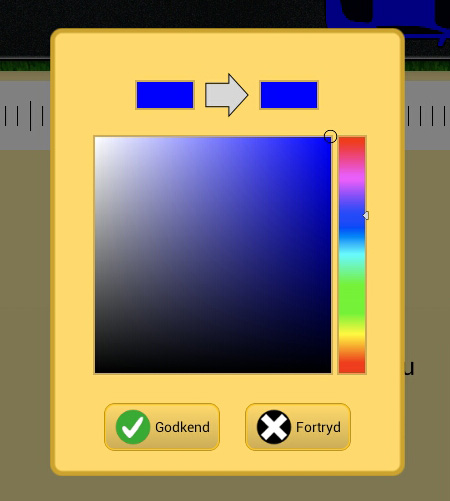
\includegraphics[width=0.49\textwidth]{sprint3/gcolorpicker}
\caption{\lstinline|GColorPicker| in Cars settings Activity}
\label{sprint3:guicomponents:fig:gcolorpicker}
\end{subfigure}

\caption{The graphics used in the game}
\label{sprint3:guicomponents:fig}
\end{figure}

\paragraph{Background color}
The main menu and setting activites were changed to use \lstinline|giraf-component|'s default background color, through the \lstinline|GetBackgroundColor()| method in the \lstinline|GComponent| class.

\paragraph{Buttons}
All menu-related buttons were changed to \lstinline|GButton|, which overrides the standard Android \lstinline|Button|.
No functionality is any different for the button, only layout.

\paragraph{Colorpicker}
The colorpicker was used for selecting car/garage colors, as mentioned in \cref{sprint3:settings}.
\lstinline|GComponent|'s \lstinline|GColorPicker| is an extension of \lstinline|GDialog|, which is an extension of Android's \lstinline|Dialog|.
The initial color of the dialog must be set by its \lstinline|SetCurrColor(int color)| method.
The new color, after choosing one in the dialog, is returned through the \lstinline|OnOkListener| interface, which provides the method \lstinline|OnOkClick(GColorPicker diag, int color)|.

\section{Evaluation}
This section contains an overview of the requirements and whether they have been fulfilled during this sprint.
Comparing \cref{sprint2:requirement_table_2} and \cref{sprint3:requirement_table} it is possible to see the progress and what has been solved during sprint 3 compared to sprint 2.
Each requirement, if fulfilled, has a link to where it is explained.
\begin{tabularenumerate}
\begin{longtable}{c|l|c|c}
\textbf{\#} & \textbf{Requirement} & \textbf{Solved} & \textbf{Link} \\
\hline
\tabenum & \begin{tabular}[l]{@{}l@{}}The game must not be a side-scrolling game,\\because the citizen must be able to see the goal\end{tabular}
 & $\surd$ & \cref{sprint1:req1} \\
\hline
\tabenum \label{sprint3:tab2:req2} & \begin{tabular}[l]{@{}l@{}}The car is controlled in such a way,\\that the vertical position of the car is relative\\ to the current loudness of the player's voice.\end{tabular}& $\surd$ & \cref{sprint2:car_control} \\
\hline
\tabenum & The goal of the game is to reach a garage & $\surd$ & \cref{sprint1:req4} \\
\hline
\tabenum \label{sprint3:tab2:req4} & When the game is won an reward should be given & $\surd$ & \cref{sprint2:won} \\
\hline
\tabenum \label{sprint3_database_req} & \begin{tabular}[l]{@{}l@{}}It must be possible\\to save and load settings for a specific profile\end{tabular} & $\surd$ & \cref{sprint3:database} \\
\hline
\tabenum \label{sprint3:req:calibrate} & It must be possible to calibrate the microphone & $\surd$ & \cref{sprint3:control_car} \\
\hline
\tabenum \label{sprint3:tab2:req7} & \begin{tabular}[l]{@{}l@{}}There is a digit between 0 and 10\\ displayed on the car as well as obstacles,\\ representing the loudness level,\\ based on its vertical position.\end{tabular} & $\surd$ & \cref{sprint2:gauges} \\
\hline
\tabenum \label{sprint3:req:picto_gauge} & \begin{tabular}[l]{@{}l@{}}Besides the scales from 0 to 10,\\ both speed and loudness have pictograms\\ illustrating some of the values on these scales.\end{tabular} & $\surd$ & \cref{sprint3:settings} \\
\hline
\tabenum \label{sprint3:tab2:req9} & \begin{tabular}[l]{@{}l@{}}It should be possible to pause the game.\\ When the game is paused,\\ a loudness-barometer is displayed next to the car,\\ further visualizing the current loudness.\end{tabular} & $\surd$ & \cref{sprint2:paused} \\
\hline
\tabenum \label{sprint3:req:speed} & \begin{tabular}[l]{@{}l@{}}Speed is alterable. The speed level\\ is represented as a digit between 0 and 10.\end{tabular} & $\surd$ & \cref{sprint3:settings} \\
\hline
\tabenum \label{sprint3:tab2:req11} & \begin{tabular}[l]{@{}l@{}}The placement and number of obstacles\\ is alterable.\end{tabular} & $\surd$ & \cref{sprint2:map_editor} \\
\hline
\tabenum \label{sprint3:tab2:req12} & \begin{tabular}[l]{@{}l@{}}The placement of obstacles should be\\ in such a way,\\ that it is possible to adapt it to both citizen\\ with tendency to speaking too loud\\ as well as those speaking too low.\end{tabular} & $\surd$ & \cref{sprint2:map_editor} \\
\hline
\tabenum \label{sprint3:tab2:req13} & \begin{tabular}[l]{@{}l@{}}The graphics need to be simple,\\ as some citizens have a low attention span\\ and are easily distracted.\end{tabular} & $\surd$ & \cref{sprint2:graphics} \\
\hline
\tabenum \label{sprint3:req:pickup_avoid} & \begin{tabular}[l]{@{}l@{}}It should be possible, in settings, to switch\\ between avoiding objects and picking objects up.\end{tabular} & $\times$ & - \\
\hline
\tabenum & \begin{tabular}[l]{@{}l@{}}When picking objects up, this is\\ linked to pictogram categories.\end{tabular} & $\times$ & - \\
\hline
\tabenum & \begin{tabular}[l]{@{}l@{}}It is important that the pickup/category\\ ''mode'' is optional, due to different capabilities\\ for each citizen.\end{tabular} & $\times$ & - \\
\hline
\caption{Requirements fulfilled after sprint 3.}
\label{sprint3:requirement_table}
\end{longtable}
\end{tabularenumerate}

\subsection{Control of the car}\label{sprint3:control_car}
It was mentioned in \cref{sprint2:eval:control_car} that the control of the car did not work properly with the current calibration.
This is regarding \cref{sprint3:req:calibrate}.
So first the calibration process was examined but no problems were found.
Then the control of the car was examined and a solution was found.
The solution to this problem was to improve the control of the car described in \cref{sprint3:stabil_car}.
So this indirect solved \cref{sprint3:req:calibrate}.
\section{Future Works}
This section contain the assignments which should be considered looking at in the next sprint.

In the next sprint the focus should be on looking at the rest of the requirements, but especially the look of the calibration in the settings.

\stefan{Er interviewet en del af future works?}

\subsection{Picking up objects}
In the next sprint it should be considered to implement a possible setting to pick up objects instead of avoiding them as stated in \cref{sprint3:req:pickup_avoid}.


\chapter{Sprint 4}\label{sprint4}
As suggested in the previous sprint the main focus of this sprint was to look at the calibration settings.
Another focus was on whether it should be able to pick up objects.
This led to an interview with speech therapist Tove Søby, where several questions were answered.
After the interview the requirements where altered and the changes applied and documented.
The picking up objects was implemented as a game mode.
The garages where removed and a finish line was inserted instead.
Sounds, to strengthen the auditory sense, was added when for instance pressing buttons and picking up objects.
At last the sprint is evaluated and found that all requirements were fulfilled.
\section{Interview}

A semi-structured interview \cite{deb} was carried out on the May 8th 2014 with the speech therapist Tove L. Søby.
Tove was the contact person who was related to the original cars project.\cite{oldcars}
We would have liked to have an interview with Tove much earlier, but communication problems throughout the project period (and a wrong email-address) caused the interview to be in the fourth sprint.

\subsection{Purpose}
The purpose of this interview was to get answers to some key questions about the fundamental purpose of the game. 
Tove is the pedagogue with the closest connection to the app and it is important that the product complies to her requirements.

\subsection{Planning}
Before the execution of the interview a number of questions and doubts was collected.


One doubt was whether the garages at the end of the track made sense, since the purpose of the game was to avoid obstacles in order to learn the citizen to talk at a specific sound level.
The garages forced the citizen to use three levels in every game played.

Is it preferred that the citizen has to avoid obstacles or is it better that they need to collect items. 

Another question was if using sounds in the game was a good idea.

A major doubt from the group prior to the interview was whether the citizen was supposed to produce a continuous sound or if it should be spoken words.
This would have a tremendous impact on the way the control of the car would need to work.

The last question was whether the text on the buttons needed to be changed to pictograms in order to make it easier for the citizen to understand.

\subsection{Result}
The result of the interview will be listed here as a list of requirements and changes to the app.

\begin{enumerate}
\item The garages need to be removed and replaced with a simple finishing line
\item Button texts need to be renamed. ``Fortsæt'' will become ``Ny tur'', and ``Menu'' will become ``Færdig''.
\item The game objective needs to be to collect items instead of avoiding them. The old game mode can be a setting.
\item Sounds at key events. Car revving at the countdown screen. Sound when collecting/colliding with things.
A jingle when the game is won.
\item All buttons in the game need to say their text when pressed.
\item The citizen is supposed to say short words when controlling the game such as ``na - na - na''. It is not supposed to be a continuous sound.
\end{enumerate}

\subsection{Requirements}\label{sprint4_req}
According to the information gathered during the interview the requirements have been updated and is available in \cref{sprint4:requirement_table}.

Changes have been made to \cref{sprint4_objective} while \cref{sprint4_sounds} and \cref{sprint4_buttonspeak} has been added.

The old requirement ``When picking objects up, this is linked to pictogram categories.'' was deleted. 
Objects that need to be picked up should use icons from a small selection of different icons (or even just one).

\begin{tabularenumerate}
\begin{longtable}{c|l|c|c}
\textbf{\#} & \textbf{Requirement} & \textbf{Solved} & \textbf{Link} \\
\hline
\tabenum & \begin{tabular}[l]{@{}l@{}}The game must not be a side-scrolling game,\\because the citizen must be able to see the goal\end{tabular}
 & $\surd$ & \cref{sprint1:req1} \\
\hline
\tabenum \label{sprint4_control} & \begin{tabular}[l]{@{}l@{}} The car is controlled in such a way,\\that the vertical position of the car is relative\\ to the current loudness of the player's voice.\end{tabular}& $\surd$ & \cref{sprint2:car_control} \\
\hline
\tabenum \label{sprint4_objective} & \begin{tabular}[l]{@{}l@{}} The goal of the game is to reach the finishing line\\ after successfully collecting all items or avoiding \\ all items (two different game modes) \end{tabular} & $\times$ & - \\
\hline
\tabenum  & When the game is won an reward should be given & $\surd$ & \cref{sprint2:won} \\
\hline
\tabenum & \begin{tabular}[l]{@{}l@{}}It must be possible\\to save and load settings for a specific profile\end{tabular} & $\surd$ & \cref{sprint3:database} \\
\hline
\tabenum & It must be possible to calibrate the microphone & $\surd$ & \cref{sprint3:control_car} \\
\hline
\tabenum  & \begin{tabular}[l]{@{}l@{}}There is a digit between 0 and 10\\ displayed on the car as well as obstacles,\\ representing the loudness level,\\ based on its vertical position.\end{tabular} & $\surd$ & \cref{sprint2:gauges} \\
\hline
\tabenum  & \begin{tabular}[l]{@{}l@{}}Besides the scales from 0 to 10,\\ both speed and loudness have pictograms\\ illustrating some of the values on these scales.\end{tabular} & $\times$ & - \\
\hline
\tabenum  & \begin{tabular}[l]{@{}l@{}}It should be possible to pause the game.\\ When the game is paused,\\ a loudness-barometer is displayed next to the car,\\ further visualizing the current loudness.\end{tabular} & $\surd$ & \cref{sprint2:paused} \\
\hline
\tabenum  & \begin{tabular}[l]{@{}l@{}}Speed is alterable. The speed level\\ is represented as a digit between 0 and 10.\end{tabular} & $\surd$ & \cref{sprint3:settings} \\
\hline
\tabenum  & \begin{tabular}[l]{@{}l@{}}The placement and number of obstacles\\ is alterable.\end{tabular} & $\surd$ & \cref{sprint2:map_editor} \\
\hline
\tabenum & \begin{tabular}[l]{@{}l@{}}The placement of obstacles should be\\ in such a way,\\ that it is possible to adapt it to both citizen\\ with tendency to speaking too loud\\ as well as those speaking too low.\end{tabular} & $\surd$ & \cref{sprint2:map_editor} \\
\hline
\tabenum & \begin{tabular}[l]{@{}l@{}}The graphics need to be simple,\\ as some citizens have a low attention span\\ and are easily distracted.\end{tabular} & $\surd$ & \cref{sprint2:graphics} \\
\hline
\tabenum  & \begin{tabular}[l]{@{}l@{}}It should be possible, in settings, to switch\\ between avoiding objects and picking objects up.\end{tabular} & $\times$ & - \\
\hline
\tabenum & \begin{tabular}[l]{@{}l@{}}It is important that the pickup/category\\ ''mode'' is optional, due to different capabilities\\ for each citizen.\end{tabular} & $\times$ & - \\
\hline
\tabenum \label{sprint4_sounds}& \begin{tabular}[l]{@{}l@{}} The game must use sounds at key events,\\ such as Car revving at the countdown screen.\\ Sound when collecting/colliding with things.\\
A jingle when the game is won.
\end{tabular}  & $\times$ & - \\
\hline
\tabenum \label{sprint4_buttonspeak}& \begin{tabular}[l]{@{}l@{}} All buttons need to read their text when pressed.
\end{tabular} & $\times$ & - \\
\hline
\caption{Requirements fulfilled after sprint 3.}
\label{sprint4:requirement_table}
\end{longtable}
\end{tabularenumerate}
\stefan{referat?}
\section{Design and Implementation}
After the interview with Tove there was some major changes to be implemented.
The new requirements are mentioned in \cref{sprint4:requirement_table} and the changes made to satisfy these requirements will be described in this section.

\begin{figure}
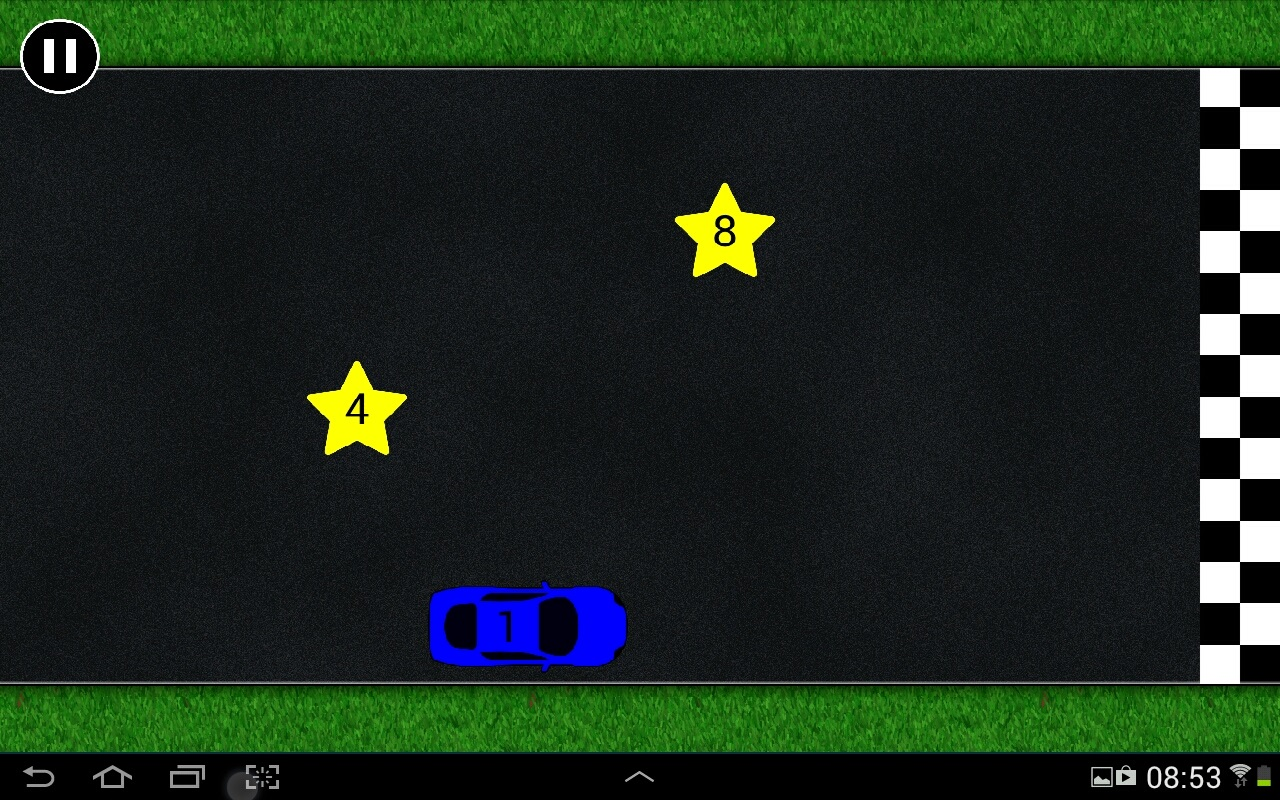
\includegraphics[width=\textwidth]{game}
\caption{The game with a finishing line as goal}
\label{game_with_finishing_line}
\end{figure}

\subsection{Game objective}\label{s4_gameobjective}
According to \cref{sprint4_objective} (see \cref{sprint4:requirement_table}) the garages had to be removed from the game and replaced with a simple finishing line.
The game also had to be changed so the items on the road had to be collected instead of avoided.
These changes introduced some changes to the logic on how to determine when the player wins.
Now it is necessary for the player to collect all items before reaching the finishing line. 
The new appearance can be seen on \cref{game_with_finishing_line}, where the new star model for items also is seen.
This new model was introduced to be able to distinguish the two game modes from each other.
Choosing between the two modes was implemented in settings as seen on \cref{gamemode}


\begin{figure}
\begin{subfigure}{0.5\textwidth}
\centering

\includegraphics{GameModeChooser}
\caption{Choosing gamemode}
\label{gamemode}
\end{subfigure}
~
\begin{subfigure}{0.5\textwidth}
\centering

\includegraphics{CarColorPicker}
\caption{Changing the color of the car}
\label{carcolor}
\end{subfigure}
\caption{Changes in settings}
\label{Settings}
\end{figure}

Because of the change away from garages it is now only necessary to choose one color for the game. 
This change was reflected in settings by only showing one colorpicker and shaping this like a car.
This car changes color according to the picked color and can be seen on \cref{carcolor}

The calibration fragment was changed slightly to blend more into the other components of the settings screen. 
A text was added to make the usage of the fragment more clear for the users.
The changed fragment as well as the complete settings screen can be seen on \cref{settings_s4}

\begin{figure}
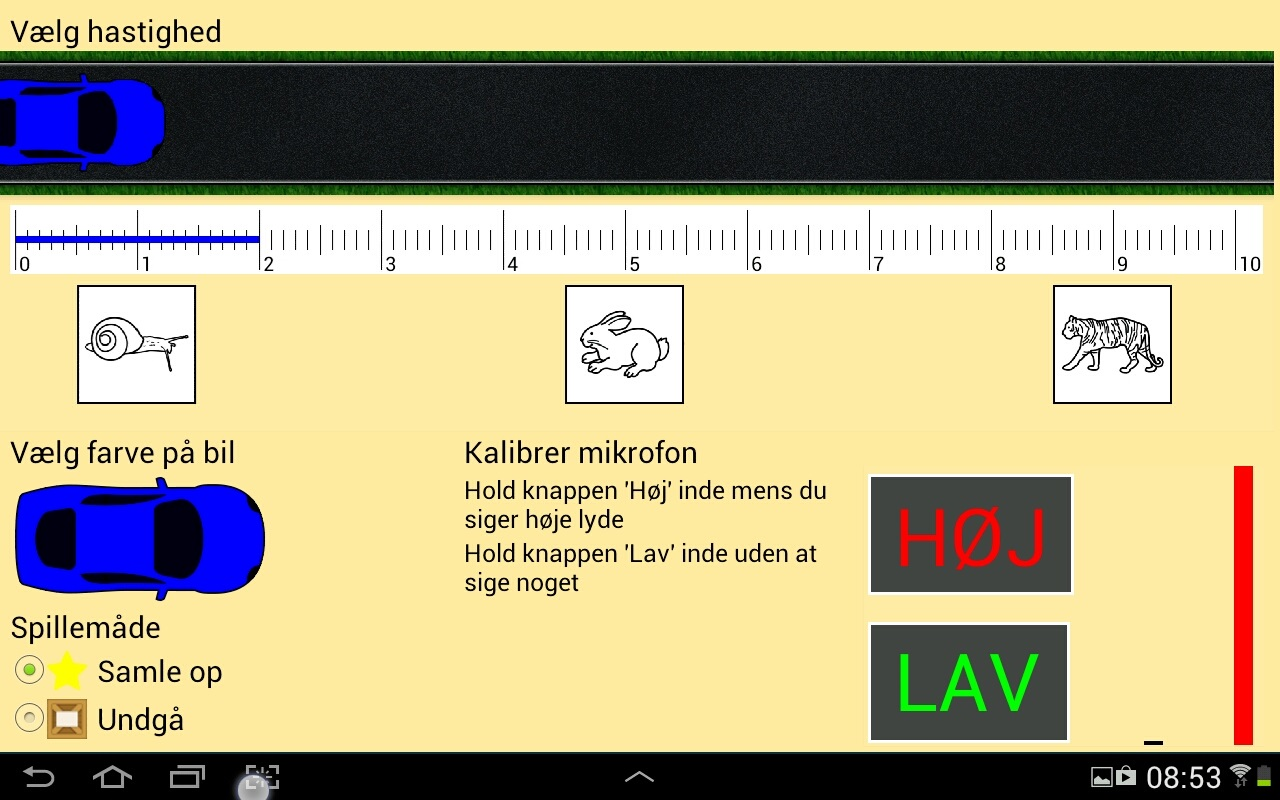
\includegraphics[width=\textwidth]{settings_s4}
\caption{The complete settings window}
\label{settings_s4}
\end{figure}

\subsection{Buttons and sounds}\label{s4_buttonsounds}
Another requirement that introduced changes to the application was \cref{sprint4_buttonspeak}.
All buttons now have to say their text when pressed and events need to have a sounds associated.

It was also a request to make the buttons look more like buttons visually.
The changes to the appearance can be seen on \cref{Buttons}, where \cref{old} shows the old appearance where a button was only the text and \cref{new} shows the new appearance where a border and background color has been added, making the button resemble a traditional button more.

\begin{figure}
\begin{subfigure}{0.5\textwidth}
\centering

\includegraphics[width=\textwidth]{oldButton}
\caption{The old appearance of the button}
\label{old}
\end{subfigure}
~
\begin{subfigure}{0.5\textwidth}
\centering

\includegraphics[width=\textwidth]{newButton}
\caption{The new appearance of the button}
\label{new}
\end{subfigure}
\caption{Changes in appearance of buttons}
\label{Buttons}
\end{figure}
\subsection{Evaluation}
This section will contain an evaluation on the fourth sprint, and how the requirements that changed after the interview (\cref{s4_interview}) have been fulfilled.

\begin{tabularenumerate}
\begin{longtable}{c|l|c|c}
\textbf{\#} & \textbf{Requirement} & \textbf{Solved} & \textbf{Link} \\
\hline
\tabenum & \begin{tabular}[l]{@{}l@{}}The game must not be a side-scrolling game,\\because the citizen must be able to see the goal\end{tabular}
 & $\surd$ & \cref{sprint1:req1} \\
\hline
\tabenum \label{sprint4_control} & \begin{tabular}[l]{@{}l@{}} The car is controlled in such a way,\\that the vertical position of the car is relative\\ to the current loudness of the player's voice.\end{tabular}& $\surd$ & \cref{sprint2:car_control} \\
\hline
\tabenum \label{sprint4_objective} & \begin{tabular}[l]{@{}l@{}} The goal of the game is to reach the finishing line\\ after successfully collecting all items or avoiding \\ all items (two different game modes) \end{tabular} & $\surd$ & \cref{s4_gameobjective} \\
\hline
\tabenum  & When the game is won an reward should be given & $\surd$ & \cref{sprint2:won} \\
\hline
\tabenum & \begin{tabular}[l]{@{}l@{}}It must be possible\\to save and load settings for a specific profile\end{tabular} & $\surd$ & \cref{sprint3:database} \\
\hline
\tabenum & It must be possible to calibrate the microphone & $\surd$ & \cref{sprint3:control_car} \\
\hline
\tabenum  & \begin{tabular}[l]{@{}l@{}}There is a digit between 0 and 10\\ displayed on the car as well as obstacles,\\ representing the loudness level,\\ based on its vertical position.\end{tabular} & $\surd$ & \cref{sprint2:gauges} \\
\hline
\tabenum  & \begin{tabular}[l]{@{}l@{}}Besides the scales from 0 to 10,\\ both speed and loudness have pictograms\\ illustrating some of the values on these scales.\end{tabular} & $\surd$ & \cref{sprint3:settings} \\
\hline
\tabenum  & \begin{tabular}[l]{@{}l@{}}It should be possible to pause the game.\\ When the game is paused,\\ a loudness-barometer is displayed next to the car,\\ further visualizing the current loudness.\end{tabular} & $\surd$ & \cref{sprint2:paused} \\
\hline
\tabenum  & \begin{tabular}[l]{@{}l@{}}Speed is alterable. The speed level\\ is represented as a digit between 0 and 10.\end{tabular} & $\surd$ & \cref{sprint3:settings} \\
\hline
\tabenum  & \begin{tabular}[l]{@{}l@{}}The placement and number of obstacles\\ is alterable.\end{tabular} & $\surd$ & \cref{sprint2:map_editor} \\
\hline
\tabenum & \begin{tabular}[l]{@{}l@{}}The placement of obstacles should be\\ in such a way,\\ that it is possible to adapt it to both citizen\\ with tendency to speaking too loud\\ as well as those speaking too low.\end{tabular} & $\surd$ & \cref{sprint2:map_editor} \\
\hline
\tabenum & \begin{tabular}[l]{@{}l@{}}The graphics need to be simple,\\ as some citizens have a low attention span\\ and are easily distracted.\end{tabular} & $\surd$ & \cref{sprint2:graphics} \\
\hline
\tabenum  & \begin{tabular}[l]{@{}l@{}}It should be possible, in settings, to switch\\ between avoiding objects and picking objects up.\end{tabular} & $\surd$ & \cref{sprint3:settings} \\
\hline
\tabenum & \begin{tabular}[l]{@{}l@{}}It is important that the pickup/category\\ ''mode'' is optional, due to different capabilities\\ for each citizen.\end{tabular} & $\times$ & - \\
\hline
\tabenum \label{sprint4_sounds}& \begin{tabular}[l]{@{}l@{}} The game must use sounds at key events,\\ such as Car revving at the countdown screen.\\ Sound when collecting/colliding with things.\\
A jingle when the game is won.
\end{tabular}  & $\surd$ & \cref{s4_buttonsounds} \\
\hline
\tabenum \label{sprint4_buttonspeak}& \begin{tabular}[l]{@{}l@{}} All buttons need to read their text when pressed.
\end{tabular} & $\surd$ & \cref{s4_buttonsounds} \\
\hline
\caption{Requirements fulfilled after sprint 3.}
\label{sprint5:requirement_table}
\end{longtable}
\end{tabularenumerate}
\section{Future Works}
As it can be seen on \cref{sprint4:requirement_table} we have fulfilled all the formal requirements gathered in the four sprints.
There is nevertheless still some things that can be improved on. 
These things will be discussed in the following.

\paragraph{Calibration}
The calibration fragment, used to calibrate the microphone, works as it is now, but its design is not as good as we would like. 
One suggestion has been to make it more like a wizard, where the fragment helps the user through the process, instead of having all the explaining text to the left of the fragment.

\paragraph{Layout in settings}
It was attempted to keep all settings on one screen to avoid the need to scroll through it
This was in the end achieved as can be seen on \cref{settings_s4}.
Unfortunately it does not fit as well on smaller screens, and even though the institution use the 10 inch format as displayed in \cref{settings_s4}, it would be a better solution if the layout would fit on all screens.

\chapter{Common Game Framework}
\section{Common Game Framework}
The cars project has been built on an existing framework as mentioned shortly in \cref{s1_redesign}. 
This made the creation of the game easier because the basic problems of game development on the android platform was already taken care of.
It was therefore relatively painless to get to the actual design of the game. 

Some project proposals at the beginning of the semester suggested making more games for the citizens.
It is therefore ideal to create a separate project that contains the framework so others can use it in future projects.
Our modified version of the framework has been moved to a new repository for this to be possible.
This repository can be a base for the development of future games in the giraf project.

In this chapter the usage of the framework will be described in order to make it easier for the students from next semester to create games in it.

\subsection{Using the framework}

\chapter{Git}
The code-base for the various applications and sub-projects that are part of the GIRAF project is quite big and requires that multiple people (possibly from different groups) can work on the same project at once.
Thus a content management system is required to manage the code and its various revisions. 
It was unanimously decided by all project groups to use Git as this content management system.
One of the reasons for using Git was that that an administration tool had already been installed on the GIRAF server.
In \cref{git:gitolite} this tool is described along with a guide to its usage.

Some of the students partaking in the project where new to the use of Git.
Because of this a \textit{''git specialist''} was chosen.
This specialist was a member of the group developing \textit{Stemmespillet}.
\mikkel{Hvor meget skal der skrives om hvor lang tid der er brugt på support?}

\section{Gitolite}\label{git:gitolite}
Gitolite is an administration tool for git repositories.
Interaction with Gitolite is done through a git repository in which all repositories are defined in one or more configuration files.
Using hooks Gitolite will create repositories when new ones are defined.
The syntax of these configuration files is described in \cref{git:gitolite:config}.

\paragraph{Accessing the server}
Each GIRAF repository is exposed through two urls.
One is read-only and is publicly available.
This allows projects to have other repo's as submodules without having write-access.
It also simplifies the servers automated build as no authentication is required.
The second url is one to which access is restricted (see \cref{git:gitolite:config}).
The two urls are as follows:
\begin{center}
\url{http://cs-cust06-int.cs.aau.dk/git-ro/} (read-only)\\
\url{http://cs-cust06-int.cs.aau.dk/git/} (read-write)
\end{center}
Each url lists a collection of repositories.
The urls for a repo is equal to appending the repo name to either of the above urls.
Connecting to these repositories can be done using LDAP authentication.
This means that the standard @student.aau.dk logins used for AAUs systems will apply to Gitolite.

\subsection{Configuration files}\label{git:gitolite:config}
As mentioned above, repositories in Gitolite are configured through a Git repository.
This repository can be found at the url below:
\begin{center}
\url{http://cs-cust06-int.cs.aau.dk/git/gitolite-admin/}
\end{center}
In the \texttt{conf} directory in the repository, a collection of files define all the GIRAF repositories.
To each repository a set of access rules apply.
These are described throughout the following section.
Note however that the access rules described below are only those applied in the course of the 2014 spring semester.
Gitolite has an online manual\footnote{\url{http://gitolite.com/gitolite/master-toc.html}} for its usage to which one should refer for any additional information.

\subsubsection{Users and groups}
In addition to defining repositories, Gitolite allows the definition of groups.
A group can be either a group of repositories or a group of users.
In the context of GIRAF only the latter is applied.
In the two files \texttt{sw6f13-groups.conf} and \texttt{sw6f14-groups.conf} the project groups for each semester are defined.
This scheme could be repeated for other semesters.
A group is defined by prefixing a name with a \textit{@} symbol, as below:
\begin{center}
\texttt{@sw600f14 = user1@student.aau.dk user2@student.aau.dk}
\end{center}
This creates a group called \texttt{@sw600f14} with two members.
The use of AAU email addresses allows the usernames to correspond directly to the LDAP authenticated users.
A group can also consist of other groups, such that a group can be created from the list of all semester groups.

\subsubsection{Multiple configuration files}
The \texttt{.conf} file loaded by Gitolite is the \texttt{gitolite.conf}.
As the list of repositories grow, multiple configuration files can be created and included.
To include a configuration file \textit{repos.conf} Gitolite has an \texttt{include} command:
\begin{center}
\texttt{include "repos.conf"}
\end{center}
This command can also be used in configuration files included using the command, and is usefull when trying to separate various types of repositories.

%Gitolite
%Common problems
% - Branches
% - Submodules
%Appendix info on setup and links to git-intro video'er

\chapter{Reflections}
When we started the semester, we had a big planning meeting with all students present.
Here we decided the overall method and structure of the project.
Since this was our first time at a collaborative project, and a big one at that, we didn't just start from scratch.
We used the experiences of those from the previous year (who in turn had also used the experiences of the year before that).

However, we did still have some things that changed during the semester, or still remain problematic and without a proper solution.

In order to give the students of next year's multi-project a better chance, by providing our experiences, we here present what we would have done in another way, or things that didn't work but we never found a proper solution to.

\paragraph{Early meetings with stakeholders} is something we wish we had, but did not.
This resulted in us establishing requirements way too late, and having to do major changes midway through, as requirements changed drastically as a result of meetings with the stakeholders.

\paragraph{Plan sprint-reviews early} in the semester.
Our first sprint-review had only 2 stakeholders present, and they had to leave early.
This was due to them being invited only shortly before the sprint-review.

It would be a good idea to establish sprint-reviews early on and invite stakeholders as soon as these are planned.
Additionally, depending on response, it could be a good idea to move sprint-reviews to fit the needs of the stakeholders, as it is really important that they can make the meeting, rather than every single person from the project-groups.

\paragraph{Requirements} was something that was determined during the first sprint by 2 groups, however, these were mostly too general and therefore not very useful.
Also, these requirements were not maintained or updated throughout the semester.
Instead, informal rules formed as a result of status meetings, individual group's meetings with stakeholders, and from sprint-reviews.

It would be a good idea to establish concrete requirements early on, and then update these as new information is gained throughout the project.

\paragraph{Status meetings} need to be short and to the point.
At first our status meetings were long and, for some, pointless.
This was due to everything being discussed by all present, even though some subjects only concerned some groups/individuals.

In the end the meetings worked a lot better, as they were very short, consisting of a short status report from each group, and if there were any problems, the concerned parties would meet or plan a meeting after the status meeting.

\paragraph{Redmine Forums} was meant as a source of discussions of non-pressing matters.
It did however not work well for this.

Firstly, the forum itself works poorly.
The layout is not very good, and its functionality very limited.
A better way of viewing what's new since last time you checked is dearly needed.

Secondly, for it to work, people need to check the forums regularly, which far from everyone did.

\paragraph{Issue-tracking} is something that never quite had the effect that we wished.
The intention was that everyone had their issue-tracker updated, so that it was possible to see what each group was currently working with.
This is hard due to the different levels of details, and in some cases complete absence, of the issues.

Another problem, which we had, is that we also like to use a real-life scrum-board, with post-its as issues.

\paragraph{Report guidelines} were a confusing matter throughout the entire semester.
One thing we should have considered from the start, is the fact that they are only guidelines, not rules.

We thought the report structure described in the guidelines as confusing and far from what we were used to, so we had a hard time adapting to this.


\label{LastNormalPage}

\appendix
% PART ******************************
\part[Appendix]{Appendix\\
	\begin{minipage}[c]{10cm}
	\centering
	\vspace{2cm}
	\normalsize{\textnormal{
		\textit{}
	}}
	\end{minipage}
}

\chapter{Code example: Run method from class RecorderThread}
\begin{lstlisting}[style=csharp,label=big_run_method, caption={Run method from the original Cars project.}]
@Override
public void run() {

System.out.println("recorderThread started");
AudioRecord recorder;
int p;
short[] audioData;
int bufferSize;
int Samplerate = 44100;
bufferSize=AudioRecord.getMinBufferSize(Samplerate,AudioFormat.CHANNEL_IN_MONO,
AudioFormat.ENCODING_PCM_16BIT)*2; //get the buffer size to use with this audio record  

recorder = new AudioRecord (AudioSource.MIC,Samplerate,AudioFormat.CHANNEL_IN_MONO,
AudioFormat.ENCODING_PCM_16BIT,bufferSize); //instantiate the AudioRecorder


recording=true; //variable to use start or stop recording
audioData = new short [bufferSize]; //short array that pcm data is put into.

while (recording) {  //loop while recording is needed
	if (recorder.getState()==android.media.AudioRecord.STATE_INITIALIZED){ // check to see if the recorder has initialized yet.
	}
	if (recorder.getRecordingState()==android.media.AudioRecord.RECORDSTATE_STOPPED){
	recorder.startRecording();  //check to see if the Recorder has stopped or is not recording, and make it record.
	}
	else {
	recorder.read(audioData,0,bufferSize); //read the PCM audio data into the audioData array
	double[] endAudioData = new double [bufferSize*2];                        
	//Now we need to decode the PCM data using the Zero Crossings Method
	//FFT fft1 = new FFT();
	short[] imgAudioData = new short [bufferSize];
	endAudioData = FFT.fft(audioData,imgAudioData, true);

	double[] magnitude = new double [bufferSize-1];
	int highestMagnitude = 0;
	for (p=2;p<(bufferSize-1)*2;p+=2){
	magnitude[p/2-1] = Math.sqrt(endAudioData[p]*endAudioData[p] + endAudioData[p+1]*endAudioData[p+1]);
	//System.out.println("magnitude = " + magnitude[p/2-1]);
	if (magnitude[p/2-1] > magnitude[highestMagnitude]){
	highestMagnitude = p/2-1;
	}
	}
	int i;
	double[] frequency = new double [bufferSize-1];  
	for (i=0 ; i<(bufferSize-1) ; i++){
	frequency[i] = ((i+1) * Samplerate/2) / (bufferSize/2);
	}

	double total = 0;
	double magnitudeTotal = 0;
	int start;
	if (highestMagnitude > 2) {
	start = -2;
	} else {
	start = 0;
	}
	int end;
	if (highestMagnitude + 2 < frequency.length) {
	end = 2;
	} else {
	end = 0;
	}
	for (i=start ; i<end ; i++){
	total += frequency[highestMagnitude+i]*magnitude[highestMagnitude+i];
	magnitudeTotal += magnitude[highestMagnitude+i];
	}
	double averageFreq = total/magnitudeTotal;
	if (averageFreq<=highestHumanPitch && magnitudeTotal>voiceSensetivity) {
	currentFrequency = (int) averageFreq;
	//System.out.println("average frequency = " + (int)averageFreq + " magnitude total = " + (int)magnitudeTotal);
	} else {
	currentFrequency = 0;
	}
	GameInfo.setCurrFreq(currentFrequency);
	}//else recorder started 
	} //while recording 

	if (recorder.getState()== android.media.AudioRecord.RECORDSTATE_RECORDING) recorder.stop(); //stop the recorder before ending the thread
	recorder.release(); //release the recorders resources
	recorder=null; //set the recorder to be garbage collected.    
}//run 
\end{lstlisting}
\chapter{Git guide for Windows}
The following section describes the setup of Git on a Windows system.
This guide was written by the Git specialist and is included for additional reference on the use of Git.
The guide was originally written in danish and has not been translated for this report, as it is not an essential part of this report.
\section{Installation af Git}
Git kan hentes på \url{http://git-scm.com/download/win}.

Under installationen kan man vælge at installere Git Bash som terminal.
Det vil jeg personligt ikke anbefale, da der findes en extension til PowerShell der laver *magi* og gør verden (på Windows) til et bedre sted.
Opsætning af dette er forklaret i \ref{gitguide:powershell} \nameref{gitguide:powershell}.
Man kan selvfølgelig også vælge at benytte en GUI - men så er man selv ude om det :P

Start den terminal du har mest lyst til at lege med (cmd.exe kan til nød anvendes her).
Tjek herefter om git er blevet korrekt installeret og at git er tilføjet til din path ved at køre:
\begin{lstlisting}
git --version
\end{lstlisting}
Terminalen skulle gerne svare med din version af git (fx \texttt{git version 1.8.3.msysgit.0}).
Hvis det ikke sker skal du tjekke at stien til git.exe (fx C:\textbackslash{}Program Files (x86)\textbackslash{}Git\textbackslash{}cmd\textbackslash{}) er i din path\footnote{Se evt \url{http://www.computerhope.com/issues/ch000549.htm}}.

\section{Opsætning af PowerShell}\label{gitguide:powershell}

PowerShell skal have rettigheder til at hente informationer som en del af følgende opsætning.
Derfor skal \texttt{ExecutionPolicy} ændres fra default (\texttt{Restricted}) til \texttt{RemoteSigned}.
Start derfor PowerShell (som administrator) og udfør følgende kommando:
\begin{lstlisting}
Set-ExecutionPolicy RemoteSigned
\end{lstlisting}

Naviger herefter til en mappe hvor git kan få lov at oprette en mappe til dig.
Her hentes lækkerierne til PowerShell ved at køre følgende kommandoer:
\begin{lstlisting}
git clone https://github.com/dahlbyk/posh-git.git
cd posh-git
.\install.ps1
\end{lstlisting}
Følg installationens vejledninger.
Slet herefter det clonede repo.

\section{ConEmu (optional - but you want it!)}

\textbf{Con}sole \textbf{Emu}lator er en wrapper til din konsol (uanset hvilken konsol du anvender) der gør din Windows konsol til alt den den skulle have været.
Blandt funktionerne kan nævnes transparency, fullscreen, global hotkeys, tabs og quake mode.
Du finder ConEmu på \url{http://sourceforge.net/projects/conemu/}.

ConEmu skal ikke installeres, men giver blot en \texttt{.7z} med executables.
Når ConEmu er startet trykkes \texttt{Win+Alt+P} for at åbne settings.
Jeg vil ikke forsøge at forklare hvor alting er at finde - det er der alt for mange muligheder til.
Følgende er blot opsætning af default terminal:
\begin{enumerate}
\item Vælg Startup -> Tasks
\item Klik på \textbf{+} i bunden af vinduet
\item Skriv et navn på din task (fx PowerShell - Git)
\item Indsæt følgende i feltet i bunden:
\begin{lstlisting}
%SystemRoot%\syswow64\WindowsPowerShell\v1.0\powershell.exe -cur_console:a
-cur_console:d:C:\Users\Mikkel\Documents\Git
\end{lstlisting}
Sidste del (\lstinline!C:\Users\Mikkel\Documents\Git!) angiver den mappe PowerShell skal startes i.
\end{enumerate}

Der findes en masse andre muligheder ift opsætning af ConEmu - bare rod lidt rundt i settings ;)

\section{Ingen indtastning af username/password}
Til sidst er her en vejledning i hvordan du slipper for at indtaste email og adgangskode hver gang du laver @push@ eller @pull@.
Et alternativ er naturligvis at anvende ssh - men det kan være problematisk på Windows.

Hent den seneste version af \textit{Windows Credential Store for Git}\footnote{\url{http://gitcredentialstore.codeplex.com/releases/view/103679}} og start den.
Det skulle gerne være nok.
Hvis konsollen (som programmet starter) bliver hængende, så skal du i din terminal navigere til den mappe du har gemt programmet i og køre:
\begin{lstlisting}
git-credential-winstore -i "C:\Program Files (x86)\Git\cmd\git.exe"
\end{lstlisting}
Husk at rette \lstinline!C:\Program Files (x86)\Git\cmd\git.exe! til stien hvor git.exe er installeret.

\chapter{Code example: Car class from project 'Cars'}
\begin{lstlisting}[style=csharp,label=car_class, caption={Car class from the original Cars project.}]
package dk.aau.cs.giraf.cars.gamecode.GameObjects;

import java.util.ArrayList;
import java.util.Random;

import javax.microedition.khronos.opengles.GL10;

import android.graphics.Color;
import android.graphics.Point;
import android.graphics.Rect;
import dk.aau.cs.giraf.cars.R;
import dk.aau.cs.giraf.cars.gamecode.GameInfo;
import dk.aau.cs.giraf.cars.gamecode.GameObject;
import dk.aau.cs.giraf.cars.gamecode.GameRenderer;
import dk.aau.cs.giraf.cars.gamecode.IDrawable;
import dk.aau.cs.giraf.cars.gamecode.IWorkable;
import dk.aau.cs.giraf.cars.gamecode.MapDivider;

public class Car extends GameObject implements IWorkable, IDrawable {
protected float xOffset = -MapDivider.obstacleWidth;
protected int yOffset = 0;
private final int mLowFreq;
private final int mHighFreq;
Point[] collisionBox;
private boolean updateCarCollisionBox = true;
private float carSpeedAsFloat;
public float carScaling = 0.7F;
private int halfObstacleHeight = (int)(MapDivider.obstacleHeight * carScaling) / 2;
private int[] colors;
private int[] bitmapIds;
private boolean[] closedColors;
private int currentColor;
	
public Car(int y, float carSpeed, int[] colors, int[] bitmapIds) {
	carSpeedAsFloat = carSpeed;
	this.yOffset = y;
	mLowFreq = GameInfo.getLowFreq();
	mHighFreq = GameInfo.getHighFreq();
		
	collisionBox = new Point[4];
	collisionBox[0] = new Point(0,0);
	collisionBox[1] = new Point(0,0);
	collisionBox[2] = new Point(0,0);
	collisionBox[3] = new Point(0,0);
	
	this.colors = colors;
	this.bitmapIds = bitmapIds;
	if (colors != null) {
		closedColors = new boolean[colors.length];
		Random rand = new Random();
		currentColor = rand.nextInt(colors.length);
	} else {
		currentColor = 0;
		this.colors = new int[] {Color.WHITE};
	}		
}
	
@Override
public void draw(GL10 gl, GameRenderer spriteBatcher) {
	if (colors[currentColor] != Color.WHITE) {
		spriteBatcher.draw(gl, bitmapIds[currentColor], new Rect(0, 0, 898, 348), new Rect( (int)xOffset, yOffset - halfObstacleHeight, (int)(MapDivider.obstacleWidth * carScaling) + (int)xOffset, yOffset + halfObstacleHeight));
	}
	else {
		spriteBatcher.draw(gl, R.drawable.car, new Rect(0, 0, 898, 348), new Rect( (int)xOffset, yOffset - halfObstacleHeight, (int)(MapDivider.obstacleWidth * carScaling) + (int)xOffset, yOffset + halfObstacleHeight));
	}
}

@Override
public void performWork() {
	updateCarCollisionBox = true;
	if (GameInfo.win == false && GameInfo.garageClosing == false && GameInfo.pause == false){
		xOffset = xOffset + carSpeedAsFloat;
	}
	int currFreq = GameInfo.getCurrFreq();
		
	if (currFreq > 0 && xOffset > -(MapDivider.obstacleWidth / 2)) {
		if (currFreq > mHighFreq && yOffset - halfObstacleHeight > MapDivider.mapYStart) {
			yOffset -= 2;
		} else if (currFreq < mLowFreq && yOffset + halfObstacleHeight < MapDivider.mapYEnd) {
			yOffset += 2;
			}
 	} else {
 		int closestLane = 0;
 		for (int i = 1; i < MapDivider.lanes; i++) {
 			if (Math.abs(MapDivider.laneCenters[i] - yOffset) <
 			Math.abs(MapDivider.laneCenters[closestLane] - yOffset)) {
 			closestLane = i;
 			}
 		}
 		int offset = MapDivider.laneCenters[closestLane] - yOffset;
		if (offset != 0) {
			if (offset > 0) {
				yOffset++;
			} else if (offset < 0) {
				yOffset--;
			}
		}
	}
}
		
public boolean CalculateCollisions(Point[] form) {
	if (updateCarCollisionBox) {
			int widthScaled = (int)(MapDivider.obstacleWidth * carScaling);
			
		collisionBox[0].x = (int)xOffset;
		collisionBox[0].y = yOffset - halfObstacleHeight;
		collisionBox[1].x = (int)xOffset;
		collisionBox[1].y = yOffset + halfObstacleHeight;
		collisionBox[2].x = widthScaled + (int)xOffset;
		collisionBox[2].y = yOffset + halfObstacleHeight;
		collisionBox[3].x = widthScaled + (int)xOffset;
		collisionBox[3].y = yOffset - halfObstacleHeight;
		
		updateCarCollisionBox = false;
	}
	if (collisionBox[0].y > form[2].y || collisionBox[1].y < form[0].y) {
		return false;
	}
	if (collisionBox[0].x > form[3].x || collisionBox[2].x < form[1].x){
		return false;
	}		
	for (int i = 0; i < 3; i++) {
		for (int j = 0; j < 3; j++) {
			if (doesLineCrossLine(collisionBox[i], collisionBox[(i + 1) % 4],
					 form[j], form[(j + 1) % 4])) {
				return true;
			}
		}
	}		
	return false;
}
private boolean doesLineCrossLine(Point line1Start, Point line1End,
								  Point line2Start, Point line2End) {
	float crossProduct1 = crossProduct(line1Start, line1End, line2Start);
	float crossProduct2 = crossProduct(line1Start, line1End, line2End);
	if ((crossProduct1 < 0 && crossProduct2 < 0) ||
			(crossProduct1 > 0 && crossProduct2 > 0)) {
		return false;
	}
	else {
		float crossProduct3 = crossProduct(line2Start, line2End, line1Start);
		float crossProduct4 = crossProduct(line2Start, line2End, line1End);
			
		if ((crossProduct3 < 0 && crossProduct4 < 0) ||
				(crossProduct3 > 0 && crossProduct4 > 0)) {
			return false;
		}
	}		
	return true;
}
private float crossProduct(Point line1Start, Point line1End,
						   Point line2Point) {
	return (line1End.x - line1Start.x) * (line2Point.y - line1End.y) -
		   (line1End.y - line1Start.y) * (line2Point.x - line1End.x);
}
	
public void resetPosition() {
	yOffset = MapDivider.mapYStart + MapDivider.totalObstacleHeight / 2 + MapDivider.totalObstacleHeight;
	xOffset = -MapDivider.obstacleWidth;
}
	
public int getColor() {
	return colors[currentColor];
}
	
public void closeColor() {
	closedColors[currentColor] = true;
	
	newColor();
}
	
public void newColor() {
	ArrayList<Integer> openColors = new ArrayList<Integer>();
	
	if (closedColors[0] == false) {
		openColors.add(0);
	}
	if (closedColors[1] == false) {
		openColors.add(1);
	}
	if (closedColors[2] == false) {
		openColors.add(2);
	}
		
	if (openColors.size() > 0) {
		Random rand = new Random();
		currentColor = penColors.get(rand.nextInt(openColors.size()));
	}
}
}
\end{lstlisting}

\chapter{Email correspondence about volume}
\subsubsection*{Email containing question for Tove, redirected by the requirements group:}\label{email_volume}
\textit{Hej sw604 aka. Requirements-gruppe,
Vi har et enkelt spørgsmål til Tove i forbindelse med vores projekt (Cars Audio Game):
"Hvis styringen af bilen i Cars var baseret på volume (dB) ville det så være brugbart?"
Samt en tilknyttet kommentar:
Vi tænker at dette kunne være relevant ift. det som Mette sagde med at nogle af børnene hviskede når der skulle råbes og omvendt.
Desuden er det meget kompliceret at få styringen til at virke med stemme-/toneleje, så vi ser dette som et kompromis for at kunne få lavet noget der virker.}

\subsubsection*{Email containing the answer from tove, from the requirements group:}
\textit{
Hej sw613,
Vi har lige været ude of snakke med Tove, og hun er syntes at det er en rigtig god idé
mvh.
sw604f14}

\chapter{Interview 3/4/2014 - Summary}
\label{app:interview-2014-04-03}\textbf{Summary written by the contact person: Mette Thomsen.}
\\
\textit{For birken er det nok for dem at bilen viser at stemmen er høj eller lav. De kunne godt lide at sætte et lyd barometer ind i spillet så børnene fx kan ses hvor højt de snakker på en skala fra 0-10. De vil gerne have et ikon der slår dette fra eller til. Det må gerne være muligt at stoppe bilen. De laver så selv koblingen med børnene mellem spil og virkeligheden. En ide de havde, var at forhindringerne var vurderet på denne skala, og at bilen så også havde et nummer der opdateret alt efter hvor bilen var. Opdeling så midten er 4-6 og alt andet er over eller under. De vil stadig gerne have mulighed for at stoppe spillet og vise lyd barometeret. De vil gerne kunne indstille antal forhindringer og hastighed. Hvis der er mange forhindringer skal bilen være mindre så der kan navigeres rundt. Lav det så simpelt som muligt! Ikke for mange detaljer på bilen eller andet da borgerne har problemer med de bliver optaget af detaljer. De øver både at borgerne skal snakke lavere og højere. Det må gerne kunne indstilles hvor forhindringerne er så et barn der snakker for højt er forhindringerne deroppe hvor bilen kører når man taler højt. På den måde bliver de tvunget til at ændre sig. De vil meget gerne kunne indstille om det handler om at undgå eller samle ting, og eventuelt begge dele. Men det skal kunne deles op. Hold alt enkelt og simpelt!}

\chapter{Interview 8/5/2014 - Summary:}
\label{interview_tove_8_5}
Tove had used the application a couple of times since the last sprint review, to see how it would perform and what could be improved.
Tove was satisfied with the settings, but the speed settings could be improved so that the number would make more sense.
Tove had forgotten how to calibrate the microphone, but remembered when showed.
Tove did find it that the children had to use too much power to steer the car, when trying to avoid the obstacles.
She would like the car control too be more sensitive.


The current application is presented.
She is impressed with the new speed settings and the way the speed barometer is used to show that visually.
But she finds the pictographs a little bit too small.
The calibration setting was not changed and is still confusing.
Tove finds that the map editor is fine.
The game gets started and Tove is impressed with the improvement of the control of the car.
Tove plays around with the speed and obstacles and is satisfied with it.
But she finds that the game gets difficult too fast when adding more obstacles.


The input volume from the player should not be a long and continuous.
The input volume should be short iterations of syllables like ''da-da-da'' or ''ba-ba-ba''.
Tove finds the game is hard with more than two obstacles.


The new idea, with picking up objects instead of avoiding them is presented and Tove likes the idea.
Tove also agrees to remove the garages, because the teacher should be in control when making the map.
Instead of the garages their should be a finish line.


The application should have sounds.
A sound when picking up an object.
A car sound when the game starts.
A voice which says the button text.
When the player wins a voice should say ''godt gået''.

When missing an object and going through to the finish line, the player should get another chance but not win.
The button text ''fortsæt'' should be changed to ''ny tur''.
The button text ''Menu'' should be changed to ''Færdig''.

\bibliography{bibliography}
\label{LastPage}
\end{document}
